\documentclass[]{book}
\usepackage{lmodern}
\usepackage{amssymb,amsmath}
\usepackage{ifxetex,ifluatex}
\usepackage{fixltx2e} % provides \textsubscript
\ifnum 0\ifxetex 1\fi\ifluatex 1\fi=0 % if pdftex
  \usepackage[T1]{fontenc}
  \usepackage[utf8]{inputenc}
\else % if luatex or xelatex
  \ifxetex
    \usepackage{mathspec}
  \else
    \usepackage{fontspec}
  \fi
  \defaultfontfeatures{Ligatures=TeX,Scale=MatchLowercase}
\fi
% use upquote if available, for straight quotes in verbatim environments
\IfFileExists{upquote.sty}{\usepackage{upquote}}{}
% use microtype if available
\IfFileExists{microtype.sty}{%
\usepackage{microtype}
\UseMicrotypeSet[protrusion]{basicmath} % disable protrusion for tt fonts
}{}
\usepackage[margin=1in]{geometry}
\usepackage{hyperref}
\hypersetup{unicode=true,
            pdftitle={Practical R for Epidemiologists},
            pdfauthor={Mark Myatt},
            pdfborder={0 0 0},
            breaklinks=true}
\urlstyle{same}  % don't use monospace font for urls
\usepackage{natbib}
\bibliographystyle{apalike}
\usepackage{color}
\usepackage{fancyvrb}
\newcommand{\VerbBar}{|}
\newcommand{\VERB}{\Verb[commandchars=\\\{\}]}
\DefineVerbatimEnvironment{Highlighting}{Verbatim}{commandchars=\\\{\}}
% Add ',fontsize=\small' for more characters per line
\usepackage{framed}
\definecolor{shadecolor}{RGB}{248,248,248}
\newenvironment{Shaded}{\begin{snugshade}}{\end{snugshade}}
\newcommand{\KeywordTok}[1]{\textcolor[rgb]{0.13,0.29,0.53}{\textbf{#1}}}
\newcommand{\DataTypeTok}[1]{\textcolor[rgb]{0.13,0.29,0.53}{#1}}
\newcommand{\DecValTok}[1]{\textcolor[rgb]{0.00,0.00,0.81}{#1}}
\newcommand{\BaseNTok}[1]{\textcolor[rgb]{0.00,0.00,0.81}{#1}}
\newcommand{\FloatTok}[1]{\textcolor[rgb]{0.00,0.00,0.81}{#1}}
\newcommand{\ConstantTok}[1]{\textcolor[rgb]{0.00,0.00,0.00}{#1}}
\newcommand{\CharTok}[1]{\textcolor[rgb]{0.31,0.60,0.02}{#1}}
\newcommand{\SpecialCharTok}[1]{\textcolor[rgb]{0.00,0.00,0.00}{#1}}
\newcommand{\StringTok}[1]{\textcolor[rgb]{0.31,0.60,0.02}{#1}}
\newcommand{\VerbatimStringTok}[1]{\textcolor[rgb]{0.31,0.60,0.02}{#1}}
\newcommand{\SpecialStringTok}[1]{\textcolor[rgb]{0.31,0.60,0.02}{#1}}
\newcommand{\ImportTok}[1]{#1}
\newcommand{\CommentTok}[1]{\textcolor[rgb]{0.56,0.35,0.01}{\textit{#1}}}
\newcommand{\DocumentationTok}[1]{\textcolor[rgb]{0.56,0.35,0.01}{\textbf{\textit{#1}}}}
\newcommand{\AnnotationTok}[1]{\textcolor[rgb]{0.56,0.35,0.01}{\textbf{\textit{#1}}}}
\newcommand{\CommentVarTok}[1]{\textcolor[rgb]{0.56,0.35,0.01}{\textbf{\textit{#1}}}}
\newcommand{\OtherTok}[1]{\textcolor[rgb]{0.56,0.35,0.01}{#1}}
\newcommand{\FunctionTok}[1]{\textcolor[rgb]{0.00,0.00,0.00}{#1}}
\newcommand{\VariableTok}[1]{\textcolor[rgb]{0.00,0.00,0.00}{#1}}
\newcommand{\ControlFlowTok}[1]{\textcolor[rgb]{0.13,0.29,0.53}{\textbf{#1}}}
\newcommand{\OperatorTok}[1]{\textcolor[rgb]{0.81,0.36,0.00}{\textbf{#1}}}
\newcommand{\BuiltInTok}[1]{#1}
\newcommand{\ExtensionTok}[1]{#1}
\newcommand{\PreprocessorTok}[1]{\textcolor[rgb]{0.56,0.35,0.01}{\textit{#1}}}
\newcommand{\AttributeTok}[1]{\textcolor[rgb]{0.77,0.63,0.00}{#1}}
\newcommand{\RegionMarkerTok}[1]{#1}
\newcommand{\InformationTok}[1]{\textcolor[rgb]{0.56,0.35,0.01}{\textbf{\textit{#1}}}}
\newcommand{\WarningTok}[1]{\textcolor[rgb]{0.56,0.35,0.01}{\textbf{\textit{#1}}}}
\newcommand{\AlertTok}[1]{\textcolor[rgb]{0.94,0.16,0.16}{#1}}
\newcommand{\ErrorTok}[1]{\textcolor[rgb]{0.64,0.00,0.00}{\textbf{#1}}}
\newcommand{\NormalTok}[1]{#1}
\usepackage{longtable,booktabs}
\usepackage{graphicx,grffile}
\makeatletter
\def\maxwidth{\ifdim\Gin@nat@width>\linewidth\linewidth\else\Gin@nat@width\fi}
\def\maxheight{\ifdim\Gin@nat@height>\textheight\textheight\else\Gin@nat@height\fi}
\makeatother
% Scale images if necessary, so that they will not overflow the page
% margins by default, and it is still possible to overwrite the defaults
% using explicit options in \includegraphics[width, height, ...]{}
\setkeys{Gin}{width=\maxwidth,height=\maxheight,keepaspectratio}
\IfFileExists{parskip.sty}{%
\usepackage{parskip}
}{% else
\setlength{\parindent}{0pt}
\setlength{\parskip}{6pt plus 2pt minus 1pt}
}
\setlength{\emergencystretch}{3em}  % prevent overfull lines
\providecommand{\tightlist}{%
  \setlength{\itemsep}{0pt}\setlength{\parskip}{0pt}}
\setcounter{secnumdepth}{5}
% Redefines (sub)paragraphs to behave more like sections
\ifx\paragraph\undefined\else
\let\oldparagraph\paragraph
\renewcommand{\paragraph}[1]{\oldparagraph{#1}\mbox{}}
\fi
\ifx\subparagraph\undefined\else
\let\oldsubparagraph\subparagraph
\renewcommand{\subparagraph}[1]{\oldsubparagraph{#1}\mbox{}}
\fi

%%% Use protect on footnotes to avoid problems with footnotes in titles
\let\rmarkdownfootnote\footnote%
\def\footnote{\protect\rmarkdownfootnote}

%%% Change title format to be more compact
\usepackage{titling}

% Create subtitle command for use in maketitle
\newcommand{\subtitle}[1]{
  \posttitle{
    \begin{center}\large#1\end{center}
    }
}

\setlength{\droptitle}{-2em}

  \title{Practical R for Epidemiologists}
    \pretitle{\vspace{\droptitle}\centering\huge}
  \posttitle{\par}
    \author{Mark Myatt}
    \preauthor{\centering\large\emph}
  \postauthor{\par}
      \predate{\centering\large\emph}
  \postdate{\par}
    \date{2018-04-21}

\usepackage{booktabs}
\usepackage{color}
\usepackage{tcolorbox}
\usepackage{float}
\graphicspath{ {images/} }

\newenvironment{rmdremind}
  {\begin{tcolorbox}[width=\textwidth, 
                     colback = {white}, 
                     title = {\textbf{Remember}}, 
                     colbacktitle = lightgray,
                     coltitle = black]
  \begin{includegraphics}[scale = 1]{remind.png}
  \begin{itemize}}
  {\end{itemize}
  \end{includegraphics}
  \end{tcolorbox}}

\newenvironment{rmdnote}
  {\begin{tcolorbox}[width=\textwidth, 
                     colback = {white}, 
                     title = {\textbf{Note}}, 
                     colbacktitle = lightgray,
                     coltitle = black]
  \begin{includegraphics}[scale = 1]{pencil.png}}
  {\end{includegraphics}
  \end{tcolorbox}}
  
\newenvironment{rmdexercise}
  {\begin{tcolorbox}[width=\textwidth, 
                     colback = {white}, 
                     title = {\textbf{Exercise}}, 
                     colbacktitle = lightgray,
                     coltitle = black]
  \begin{includegraphics}[scale = 1]{exercise.png}}
  {\end{includegraphics}
  \end{tcolorbox}}
  
\newenvironment{rmdinfo}
  {\begin{tcolorbox}[width=\textwidth, 
                     colback = {white}, 
                     title = {\textbf{Info}}, 
                     colbacktitle = lightgray,
                     coltitle = black]
  \begin{includegraphics}[scale = 1]{info.png}}
  {\end{includegraphics}
  \end{tcolorbox}}  
  
\newenvironment{rmdwarning}
  {\begin{tcolorbox}[width=\textwidth, 
                     colback = {white}, 
                     title = {\textbf{Warning}}, 
                     colbacktitle = lightgray,
                     coltitle = black]
  \begin{includegraphics}[scale = 1]{warning.png}}
  {\end{includegraphics}
  \end{tcolorbox}}

\newenvironment{rmddownload}
  {\begin{tcolorbox}[width=\textwidth, 
                     colback = {white}, 
                     title = {\textbf{Download}}, 
                     colbacktitle = lightgray,
                     coltitle = black]
  \begin{includegraphics}[scale = 1]{download.png}}
  {\end{includegraphics}
  \end{tcolorbox}}

\usepackage{amsthm}
\newtheorem{theorem}{Theorem}[chapter]
\newtheorem{lemma}{Lemma}[chapter]
\theoremstyle{definition}
\newtheorem{definition}{Definition}[chapter]
\newtheorem{corollary}{Corollary}[chapter]
\newtheorem{proposition}{Proposition}[chapter]
\theoremstyle{definition}
\newtheorem{example}{Example}[chapter]
\theoremstyle{definition}
\newtheorem{exercise}{Exercise}[chapter]
\theoremstyle{remark}
\newtheorem*{remark}{Remark}
\newtheorem*{solution}{Solution}
\begin{document}
\maketitle

{
\setcounter{tocdepth}{1}
\tableofcontents
}
\hypertarget{chapter1}{%
\chapter{Introduction}\label{chapter1}}

\hypertarget{introducing-r}{%
\section{Introducing R}\label{introducing-r}}

\texttt{R} is a system for data manipulation, calculation, and graphics.
It provides:

\begin{itemize}
\item
  Facilities for data handling and storage
\item
  A large collection of tools for data analysis
\item
  Graphical facilities for data analysis and display
\item
  A simple but powerful programming language
\end{itemize}

\texttt{R} is often described as an environment for working with data.
This is in contrast to a \emph{package} which is a collection of very
specific tools. \texttt{R} is not strictly a statistics system but a
system that provides many classical and modern statistical procedures as
part of a broader data-analysis tool. This is an important difference
between \texttt{R} and other statistical systems. In \texttt{R} a
statistical analysis is usually performed as a series of steps with
intermediate results being stored in objects. Systems such as
\texttt{SPSS} and \texttt{SAS} provide copious output from (e.g.) a
regression analysis whereas \texttt{R} will give minimal output and
store the results of a fit for subsequent interrogation or use with
other \texttt{R} functions. This means that \texttt{R} can be tailored
to produce exactly the analysis and results that you want rather than
produce an analysis designed to fit all situations.

\texttt{R} is a language based product. This means that you interact
with \texttt{R} by typing commands such as:

\begin{Shaded}
\begin{Highlighting}[]
\KeywordTok{table}\NormalTok{(SEX, LIFE)}
\end{Highlighting}
\end{Shaded}

rather than by using menus, dialog boxes, selection lists, and buttons.
This may seem to be a drawback but it means that the system is
considerably more flexible than one that relies on menus, buttons, and
boxes. It also means that every stage of your data management and
analysis can be recorded and edited and re-run at a later date. It also
provides an audit trail for quality control purposes.

\texttt{R} is available under UNIX (including Linux), the Macintosh
operating system OS X, and Microsoft Windows. The method used for
starting \texttt{R} will vary from system to system. On UNIX systems you
may need to issue the \texttt{R} command in a terminal session or click
on an icon or menu option if your system has a windowing system. On
Macintosh systems \texttt{R} will be available as an application but can
also be run in a terminal session. On Microsoft Windows systems there
will usually be an icon on the Start menu or the desktop.

\texttt{R} is an open source system and is available under the \emph{GNU
general public license} (GPL) which means that it is available for free
but that there are some restrictions on how you are allowed to
distribute the system and how you may charge for bespoke data analysis
solutions written using the \texttt{R} system. Details of the general
public license are available from
\url{http://www.gnu.org/copyleft/gpl.html}.

\texttt{R} is available for download from
\url{http://www.r-project.org/}.

This is also the best place to get extension packages and documentation.
You may also subscribe to the \texttt{R} mailing lists from this site.
\texttt{R} is supported through mailing lists. The level of support is
at least as good as for commercial packages. It is typical to have
queries answered in a matter of a few hours.

Even though \texttt{R} is a free package it is more powerful than most
commercial packages. Many of the modern procedures found in commercial
packages were first developed and tested using \texttt{R} or
\textbf{S-Plus} (the commercial equivalent of \texttt{R}).

When you start \texttt{R} it will issue a prompt when it expects user
input. The default prompt is:

\begin{verbatim}
>
\end{verbatim}

This is where you type commands that call functions that instruct
\texttt{R} to (e.g.) read a data file, recode data, produce a table, or
fit a regression. For example:

\begin{verbatim}
   > table(SEX, LIFE)
\end{verbatim}

If a command you type is not complete then the prompt will change to:

\begin{verbatim}
+
\end{verbatim}

on subsequent lines until the command is complete:

\begin{verbatim}
> table(
+ SEX, LIFE +)
\end{verbatim}

The \texttt{\textgreater{}} and \texttt{+} prompts are not shown in the
example commands in the rest of this material.

The example commands in this material are often broken into shorter
lines and indented for ease of understanding. The code still works as
lines are split in places where \texttt{R} knows that a line is not
complete. For example:

\begin{Shaded}
\begin{Highlighting}[]
\KeywordTok{table}\NormalTok{(SEX,}
\NormalTok{      LIFE)}
\end{Highlighting}
\end{Shaded}

could be entered on a single line as:

\begin{Shaded}
\begin{Highlighting}[]
\KeywordTok{table}\NormalTok{(SEX, LIFE)}
\end{Highlighting}
\end{Shaded}

In this example \texttt{R} knows that the command is not complete until
the brackets are closed. The following example could also be written on
one line:

\begin{Shaded}
\begin{Highlighting}[]
\NormalTok{salex.lreg.coeffs <-}
\StringTok{  }\KeywordTok{coef}\NormalTok{(}\KeywordTok{summary}\NormalTok{(salex.lreg))}
\end{Highlighting}
\end{Shaded}

In this case \texttt{R} knows that the \texttt{\textless{}-} operator at
the end of the first line needs further input.

\texttt{R} maintains a history of previous commands. These can be
recalled and edited using the up and down arrow keys.

Output that has scrolled off the top of the output / command window can
be recalled using the window or terminal scroll bars.

Output can be saved using the \texttt{sink()} function with a file name:
\texttt{sink("results.out")} to start recording output. Use the
\texttt{sink()} function without a file name to stop recording output:
\texttt{sink()}

You can also use clipboard functions such as copy and paste to (e.g.)
copy and then paste selected chunks of output into an editor or word
processor running alongside \texttt{R}.

All the sample data files used in the exercises in this manual are space
delimited text files using the general format:

\begin{verbatim}
   ID AGE IQ
   1 39 94
   2 41 89
   3 42 83
   4 30 99
   5 35 94
   6 44 90
   7 31 94
   8 39 87
\end{verbatim}

\texttt{R} has facilities for working with files in different formats
including (through the use of extension packages) \textbf{ODBC} (open
database connectivity) and \textbf{SQL} data sources, \textbf{EpiInfo},
\textbf{EpiData}, \textbf{Minitab}, \textbf{SPSS}, \textbf{SAS},
\textbf{S-Plus}, and \textbf{Stata} format files.

\hypertarget{retrieving-data}{%
\section{Retrieving data}\label{retrieving-data}}

All of the exercises in this manual assume that the necessary data files
are located in the current working directory. All of the data files that
you require to follow this material are in a ZIP archive that can be
downloaded from:

\url{http://www.brixtonhealth.com/prfe/prfe.zip}

A command such as:

\begin{Shaded}
\begin{Highlighting}[]
\KeywordTok{read.table}\NormalTok{(}\StringTok{"data/fem.dat"}\NormalTok{, }\DataTypeTok{header =} \OtherTok{TRUE}\NormalTok{)}
\end{Highlighting}
\end{Shaded}

retrieves the data stored in the file named \texttt{fem.dat} which is
stored in the \texttt{data} folder.

To retrieve data that is stored in files outside a different directory
you need to specify the full path to the file. For example:

\begin{Shaded}
\begin{Highlighting}[]
\KeywordTok{read.table}\NormalTok{(}\StringTok{"~/example/fem.dat"}\NormalTok{, }\DataTypeTok{header =} \OtherTok{TRUE}\NormalTok{)}
\end{Highlighting}
\end{Shaded}

will retrieve the data stored in the file named \texttt{fem.dat} stored
in the \texttt{example} directory under the user's home directory on
UNIX, Linux, and OS X systems.

\texttt{R} follows many UNIX operating and naming conventions including
the use of the backslash (\texttt{\textbackslash{}}) character to
specify special characters in strings (e.g.~using
\texttt{\textbackslash{}n} to specify a new line in printed output).
Windows uses the backslash (\texttt{\textbackslash{}}) character to
separate directory and file names in paths. This means that Windows
users need to escape any backslashes in file paths using an additional
backslash character. For example:

\begin{Shaded}
\begin{Highlighting}[]
\KeywordTok{read.table}\NormalTok{(}\StringTok{"c:}\CharTok{\textbackslash{}\textbackslash{}}\StringTok{example}\CharTok{\textbackslash{}\textbackslash{}}\StringTok{fem.dat"}\NormalTok{, }\DataTypeTok{header =} \OtherTok{TRUE}\NormalTok{)}
\end{Highlighting}
\end{Shaded}

will retrieve the data that is stored in the file named \texttt{fem.dat}
which is stored in the \texttt{example} directory off the root directory
of the \texttt{C:} drive. The Windows version of \texttt{R} also allows
you to specify UNIX-style path names (i.e.~using the forward slash
(\texttt{/}) character as a separator in file paths). For example:

\begin{Shaded}
\begin{Highlighting}[]
\KeywordTok{read.table}\NormalTok{(}\StringTok{"c:/example/fem.dat"}\NormalTok{, }\DataTypeTok{header =} \OtherTok{TRUE}\NormalTok{)}
\end{Highlighting}
\end{Shaded}

Path names may include shortcut characters such as:

\begin{longtable}[]{@{}cl@{}}
\toprule
\texttt{.} & The current working directory\tabularnewline
\texttt{..} & Up one level in the directory tree\tabularnewline
\texttt{\textasciitilde{}} & The user's home directory (on UNIX-based
systems)\tabularnewline
\bottomrule
\end{longtable}

\texttt{R} also allows you to retrieve files from any location that may
be represented by a standard \texttt{uniform\ resource\ locator\ (URL)}
string. For example:

\begin{Shaded}
\begin{Highlighting}[]
\KeywordTok{read.table}\NormalTok{(}\StringTok{"file://~/example/fem.dat"}\NormalTok{, }\DataTypeTok{header =} \OtherTok{TRUE}\NormalTok{)}
\end{Highlighting}
\end{Shaded}

will retrieve the data stored in the file named \texttt{fem.dat} stored
in the \texttt{example} directory under the users home directory on
UNIX-based systems.

All of the data files used in this section are stored in the
\texttt{/data} directory of this guide's GitLab repository
(\url{https://git.validmeasures.org/datahub/datahubguide/tree/master/data}).
This means, for example, that you can use the \texttt{read.table()}
function specifying

``\url{https://git.validmeasures.org/datahub/datahubguide/tree/master/data/fem.dat}''

as the \texttt{URL} to retrieve the data that is stored in the file
named \texttt{fem.dat} which is stored in the \texttt{/data} directory
of this guide's GitLab repository.

\hypertarget{exercise1}{%
\chapter{Getting acquainted with R}\label{exercise1}}

In this exercise we will use \texttt{R} to read a dataset and produce
some descriptive statistics, produce some charts, and perform some
simple statistical inference. The aim of the exercise is for you to
become familiar with \texttt{R} and some basic \texttt{R} functions and
objects.

The first thing we will do, after starting \texttt{R}, is issue a
command to retrieve an example dataset:

\begin{Shaded}
\begin{Highlighting}[]
\NormalTok{fem <-}\StringTok{ }\KeywordTok{read.table}\NormalTok{(}\StringTok{"fem.dat"}\NormalTok{, }\DataTypeTok{header =} \OtherTok{TRUE}\NormalTok{)}
\end{Highlighting}
\end{Shaded}

This command illustrates some key things about the way \texttt{R} works.

We are instructing \texttt{R} to assign (using the \texttt{\textless{}-}
operator) the output of the \texttt{read.table()} function to an object
called \texttt{fem}.

The \texttt{fem} object will contain the data held in the file
\texttt{fem.dat} as an \texttt{R} data.frame object:

\begin{Shaded}
\begin{Highlighting}[]
\KeywordTok{class}\NormalTok{(fem)}
\end{Highlighting}
\end{Shaded}

\begin{verbatim}
## [1] "data.frame"
\end{verbatim}

You can inspect the contents of the \texttt{fem} data.frame (or any
other \texttt{R} object) just by typing its name:

\begin{Shaded}
\begin{Highlighting}[]
\NormalTok{fem}
\end{Highlighting}
\end{Shaded}

\begin{verbatim}
##   ID AGE IQ ANX DEP SLP SEX LIFE    WT
## 1  1  39 94   2   2   2   1    1  2.23
## 2  2  41 89   2   2   2   1    1  1.00
## 3  3  42 83   3   3   2   1    1  1.82
## 4  4  30 99   2   2   2   1    1 -1.18
## 5  5  35 94   2   1   1   1    2 -0.14
## 6  6  44 90  NA   1   2   2    2  0.41
\end{verbatim}

Note that the \texttt{fem} object is built from other objects. These are
the named vectors (columns) in the dataset:

\begin{Shaded}
\begin{Highlighting}[]
\KeywordTok{names}\NormalTok{(fem)}
\end{Highlighting}
\end{Shaded}

\begin{verbatim}
## [1] "ID"   "AGE"  "IQ"   "ANX"  "DEP"  "SLP"  "SEX"  "LIFE" "WT"
\end{verbatim}

The \texttt{{[}1{]}} displayed before the column names refers to the
numbered position of the first name in the output. These positions are
known as indexes and can be used to refer to individual items. For
example:

\begin{Shaded}
\begin{Highlighting}[]
\KeywordTok{names}\NormalTok{(fem)[}\DecValTok{1}\NormalTok{]}
\end{Highlighting}
\end{Shaded}

\begin{verbatim}
## [1] "ID"
\end{verbatim}

\begin{Shaded}
\begin{Highlighting}[]
\KeywordTok{names}\NormalTok{(fem)[}\DecValTok{8}\NormalTok{]}
\end{Highlighting}
\end{Shaded}

\begin{verbatim}
## [1] "LIFE"
\end{verbatim}

\begin{Shaded}
\begin{Highlighting}[]
\KeywordTok{names}\NormalTok{(fem)[}\DecValTok{2}\OperatorTok{:}\DecValTok{4}\NormalTok{]}
\end{Highlighting}
\end{Shaded}

\begin{verbatim}
## [1] "AGE" "IQ"  "ANX"
\end{verbatim}

The data consist of 118 records:

\begin{Shaded}
\begin{Highlighting}[]
\KeywordTok{nrow}\NormalTok{(fem)}
\end{Highlighting}
\end{Shaded}

\begin{verbatim}
## [1] 118
\end{verbatim}

each with nine variables:

\begin{Shaded}
\begin{Highlighting}[]
\KeywordTok{ncol}\NormalTok{(fem)}
\end{Highlighting}
\end{Shaded}

\begin{verbatim}
## [1] 9
\end{verbatim}

for female psychiatric patients.

The columns in the dataset are:

\begin{longtable}[]{@{}ll@{}}
\toprule
\begin{minipage}[b]{0.14\columnwidth}\raggedright
\textbf{ID}\strut
\end{minipage} & \begin{minipage}[b]{0.69\columnwidth}\raggedright
Patient ID\strut
\end{minipage}\tabularnewline
\midrule
\endhead
\begin{minipage}[t]{0.14\columnwidth}\raggedright
\textbf{AGE}\strut
\end{minipage} & \begin{minipage}[t]{0.69\columnwidth}\raggedright
Age in years\strut
\end{minipage}\tabularnewline
\begin{minipage}[t]{0.14\columnwidth}\raggedright
\textbf{IQ}\strut
\end{minipage} & \begin{minipage}[t]{0.69\columnwidth}\raggedright
IQ score\strut
\end{minipage}\tabularnewline
\begin{minipage}[t]{0.14\columnwidth}\raggedright
\textbf{ANX}\strut
\end{minipage} & \begin{minipage}[t]{0.69\columnwidth}\raggedright
Anxiety (1=none, 2=mild, 3=moderate, 4=severe)\strut
\end{minipage}\tabularnewline
\begin{minipage}[t]{0.14\columnwidth}\raggedright
\textbf{DEP}\strut
\end{minipage} & \begin{minipage}[t]{0.69\columnwidth}\raggedright
Depression (1=none, 2=mild, 3=moderate or severe)\strut
\end{minipage}\tabularnewline
\begin{minipage}[t]{0.14\columnwidth}\raggedright
\textbf{SLP}\strut
\end{minipage} & \begin{minipage}[t]{0.69\columnwidth}\raggedright
Sleeping normally (1=yes, 2=no)\strut
\end{minipage}\tabularnewline
\begin{minipage}[t]{0.14\columnwidth}\raggedright
\textbf{SEX}\strut
\end{minipage} & \begin{minipage}[t]{0.69\columnwidth}\raggedright
Lost interest in sex (1=yes, 2=no)\strut
\end{minipage}\tabularnewline
\begin{minipage}[t]{0.14\columnwidth}\raggedright
\textbf{LIFE}\strut
\end{minipage} & \begin{minipage}[t]{0.69\columnwidth}\raggedright
Considered suicide (1=yes, 2=no)\strut
\end{minipage}\tabularnewline
\begin{minipage}[t]{0.14\columnwidth}\raggedright
\textbf{WT}\strut
\end{minipage} & \begin{minipage}[t]{0.69\columnwidth}\raggedright
Weight change (kg) in previous 6 months\strut
\end{minipage}\tabularnewline
\bottomrule
\end{longtable}

The first ten records of the \texttt{fem} data.frame are:

\begin{verbatim}
##    ID AGE  IQ ANX DEP SLP SEX LIFE    WT
## 1   1  39  94   2   2   2   1    1  2.23
## 2   2  41  89   2   2   2   1    1  1.00
## 3   3  42  83   3   3   2   1    1  1.82
## 4   4  30  99   2   2   2   1    1 -1.18
## 5   5  35  94   2   1   1   1    2 -0.14
## 6   6  44  90  NA   1   2   2    2  0.41
## 7   7  31  94   2   2  NA   1    1 -0.68
## 8   8  39  87   3   2   2   1    2  1.59
## 9   9  35 -99   3   2   2   1    1 -0.55
## 10 10  33  92   2   2   2   1    1  0.36
\end{verbatim}

You may check this by asking \texttt{R} to display all columns of the
first ten records in the \texttt{fem} data.frame:

\begin{Shaded}
\begin{Highlighting}[]
\NormalTok{fem[}\DecValTok{1}\OperatorTok{:}\DecValTok{10}\NormalTok{, ]}
\end{Highlighting}
\end{Shaded}

\begin{verbatim}
##    ID AGE  IQ ANX DEP SLP SEX LIFE    WT
## 1   1  39  94   2   2   2   1    1  2.23
## 2   2  41  89   2   2   2   1    1  1.00
## 3   3  42  83   3   3   2   1    1  1.82
## 4   4  30  99   2   2   2   1    1 -1.18
## 5   5  35  94   2   1   1   1    2 -0.14
## 6   6  44  90  NA   1   2   2    2  0.41
## 7   7  31  94   2   2  NA   1    1 -0.68
## 8   8  39  87   3   2   2   1    2  1.59
## 9   9  35 -99   3   2   2   1    1 -0.55
## 10 10  33  92   2   2   2   1    1  0.36
\end{verbatim}

The space after the comma is optional. You can think of it as a
\emph{placeholder} for where you would specify the indexes for columns
you wanted to display. For example:

\begin{Shaded}
\begin{Highlighting}[]
\NormalTok{fem[}\DecValTok{1}\OperatorTok{:}\DecValTok{10}\NormalTok{,}\DecValTok{2}\OperatorTok{:}\DecValTok{4}\NormalTok{]}
\end{Highlighting}
\end{Shaded}

displays the first ten rows and the second, third and fourth columns of
the \texttt{fem} data.frame:

\begin{verbatim}
##    AGE  IQ ANX
## 1   39  94   2
## 2   41  89   2
## 3   42  83   3
## 4   30  99   2
## 5   35  94   2
## 6   44  90  NA
## 7   31  94   2
## 8   39  87   3
## 9   35 -99   3
## 10  33  92   2
\end{verbatim}

\texttt{NA} is a special value meaning \emph{not available} or
\emph{missing}.

You can access the contents of a single column by name:

\begin{Shaded}
\begin{Highlighting}[]
\NormalTok{fem}\OperatorTok{$}\NormalTok{IQ}
\end{Highlighting}
\end{Shaded}

\begin{verbatim}
##   [1]  94  89  83  99  94  90  94  87 -99  92  92  94  91  86  90 -99  91
##  [18]  82  86  88  97  96  95  87 103 -99  91  87  91  89  92  84  94  92
##  [35]  96  96  86  92 102  82  92  90  92  88  98  93  90  91 -99  92  92
##  [52]  91  91  86  95  91  96 100  99  89  89  98  98 103  91  91  94  91
##  [69]  85  92  96  90  87  95  95  87  95  88  94 -99 -99  87  92  86  93
##  [86]  92 106  93  95  95  92  98  92  88  85  92  84  92  91  86  92  89
## [103] -99  96  97  92  92  98  91  91  89  94  90  96  87  86  89 -99
\end{verbatim}

\begin{Shaded}
\begin{Highlighting}[]
\NormalTok{fem}\OperatorTok{$}\NormalTok{IQ[}\DecValTok{1}\OperatorTok{:}\DecValTok{10}\NormalTok{]}
\end{Highlighting}
\end{Shaded}

\begin{verbatim}
##  [1]  94  89  83  99  94  90  94  87 -99  92
\end{verbatim}

The \texttt{\$} sign is used to separate the name of the data.frame and
the name of the column of interest. Note that \texttt{R} is
case-sensitive so that \texttt{IQ} and \texttt{iq} are
\textbf{\emph{not}} the same.

You can also access rows, columns, and individual cells by specifying
row and column positions. For example, the \texttt{IQ} column is the
third column in the \texttt{fem} data.frame:

\begin{Shaded}
\begin{Highlighting}[]
\NormalTok{fem[ ,}\DecValTok{3}\NormalTok{]}
\end{Highlighting}
\end{Shaded}

\begin{verbatim}
##   [1]  94  89  83  99  94  90  94  87 -99  92  92  94  91  86  90 -99  91
##  [18]  82  86  88  97  96  95  87 103 -99  91  87  91  89  92  84  94  92
##  [35]  96  96  86  92 102  82  92  90  92  88  98  93  90  91 -99  92  92
##  [52]  91  91  86  95  91  96 100  99  89  89  98  98 103  91  91  94  91
##  [69]  85  92  96  90  87  95  95  87  95  88  94 -99 -99  87  92  86  93
##  [86]  92 106  93  95  95  92  98  92  88  85  92  84  92  91  86  92  89
## [103] -99  96  97  92  92  98  91  91  89  94  90  96  87  86  89 -99
\end{verbatim}

\begin{Shaded}
\begin{Highlighting}[]
\NormalTok{fem[}\DecValTok{9}\NormalTok{, ]}
\end{Highlighting}
\end{Shaded}

\begin{verbatim}
##   ID AGE  IQ ANX DEP SLP SEX LIFE    WT
## 9  9  35 -99   3   2   2   1    1 -0.55
\end{verbatim}

\begin{Shaded}
\begin{Highlighting}[]
\NormalTok{fem[}\DecValTok{9}\NormalTok{,}\DecValTok{3}\NormalTok{]}
\end{Highlighting}
\end{Shaded}

\begin{verbatim}
## [1] -99
\end{verbatim}

There are missing values in the \texttt{IQ} column which are all coded
as \textbf{-99}. Before proceeding we must set these to the special
\texttt{NA} value:

\begin{Shaded}
\begin{Highlighting}[]
\NormalTok{fem}\OperatorTok{$}\NormalTok{IQ[fem}\OperatorTok{$}\NormalTok{IQ }\OperatorTok{==}\StringTok{ }\DecValTok{-99}\NormalTok{] <-}\StringTok{ }\OtherTok{NA}
\end{Highlighting}
\end{Shaded}

The term inside the square brackets is also an index. This type of index
is used to refer to subsets of data held in an object that meet a
particular condition. In this case we are instructing \texttt{R} to set
the contents of the \texttt{IQ} variable to \texttt{NA} if the contents
of the \texttt{IQ} variable is \textbf{-99}.

Check that this has worked:

\begin{Shaded}
\begin{Highlighting}[]
\NormalTok{fem}\OperatorTok{$}\NormalTok{IQ}
\end{Highlighting}
\end{Shaded}

\begin{verbatim}
##   [1]  94  89  83  99  94  90  94  87  NA  92  92  94  91  86  90  NA  91
##  [18]  82  86  88  97  96  95  87 103  NA  91  87  91  89  92  84  94  92
##  [35]  96  96  86  92 102  82  92  90  92  88  98  93  90  91  NA  92  92
##  [52]  91  91  86  95  91  96 100  99  89  89  98  98 103  91  91  94  91
##  [69]  85  92  96  90  87  95  95  87  95  88  94  NA  NA  87  92  86  93
##  [86]  92 106  93  95  95  92  98  92  88  85  92  84  92  91  86  92  89
## [103]  NA  96  97  92  92  98  91  91  89  94  90  96  87  86  89  NA
\end{verbatim}

We can now compare the groups who have and have not considered suicide.
For example:

\begin{Shaded}
\begin{Highlighting}[]
\KeywordTok{by}\NormalTok{(fem}\OperatorTok{$}\NormalTok{IQ, fem}\OperatorTok{$}\NormalTok{LIFE, summary)}
\end{Highlighting}
\end{Shaded}

Look at the help for the \texttt{by()} function:

\begin{Shaded}
\begin{Highlighting}[]
\KeywordTok{help}\NormalTok{(by)}
\end{Highlighting}
\end{Shaded}

Note that you may use \texttt{?by} as a shortcut for \texttt{help(by)}.

The \texttt{by()} function applies another function (in this case the
\texttt{summary()} function) to a column in a data.frame (in this case
\texttt{fem\$IQ}) split by the value of another variable (in this case
\texttt{fem\$LIFE}).

It can be tedious to always have to specify a data.frame each time we
want to use a particular variable. We can fix this problem by
`attaching' the data.frame:

\begin{Shaded}
\begin{Highlighting}[]
\KeywordTok{attach}\NormalTok{(fem)}
\end{Highlighting}
\end{Shaded}

\begin{verbatim}
## The following objects are masked from fem (pos = 4):
## 
##     AGE, ANX, DEP, ID, IQ, LIFE, SEX, SLP, WT
\end{verbatim}

We can now refer to the columns in the \texttt{fem} data.frame without
having to specify the name of the data.frame. This time we will produce
summary statistics for \texttt{WT} by \texttt{LIFE}:

\begin{Shaded}
\begin{Highlighting}[]
\KeywordTok{by}\NormalTok{(WT, LIFE, summary)}
\end{Highlighting}
\end{Shaded}

\begin{verbatim}
## LIFE: 1
##    Min. 1st Qu.  Median    Mean 3rd Qu.    Max.    NA's 
## -2.2300 -0.2700  1.0000  0.7867  1.7300  3.7700       4 
## -------------------------------------------------------- 
## LIFE: 2
##    Min. 1st Qu.  Median    Mean 3rd Qu.    Max.    NA's 
## -1.6800 -0.4500  0.6400  0.6404  1.5000  2.9500       7
\end{verbatim}

We can view the same data as a box and whisker plot:

\begin{Shaded}
\begin{Highlighting}[]
\KeywordTok{boxplot}\NormalTok{(WT }\OperatorTok{~}\StringTok{ }\NormalTok{LIFE)}
\end{Highlighting}
\end{Shaded}

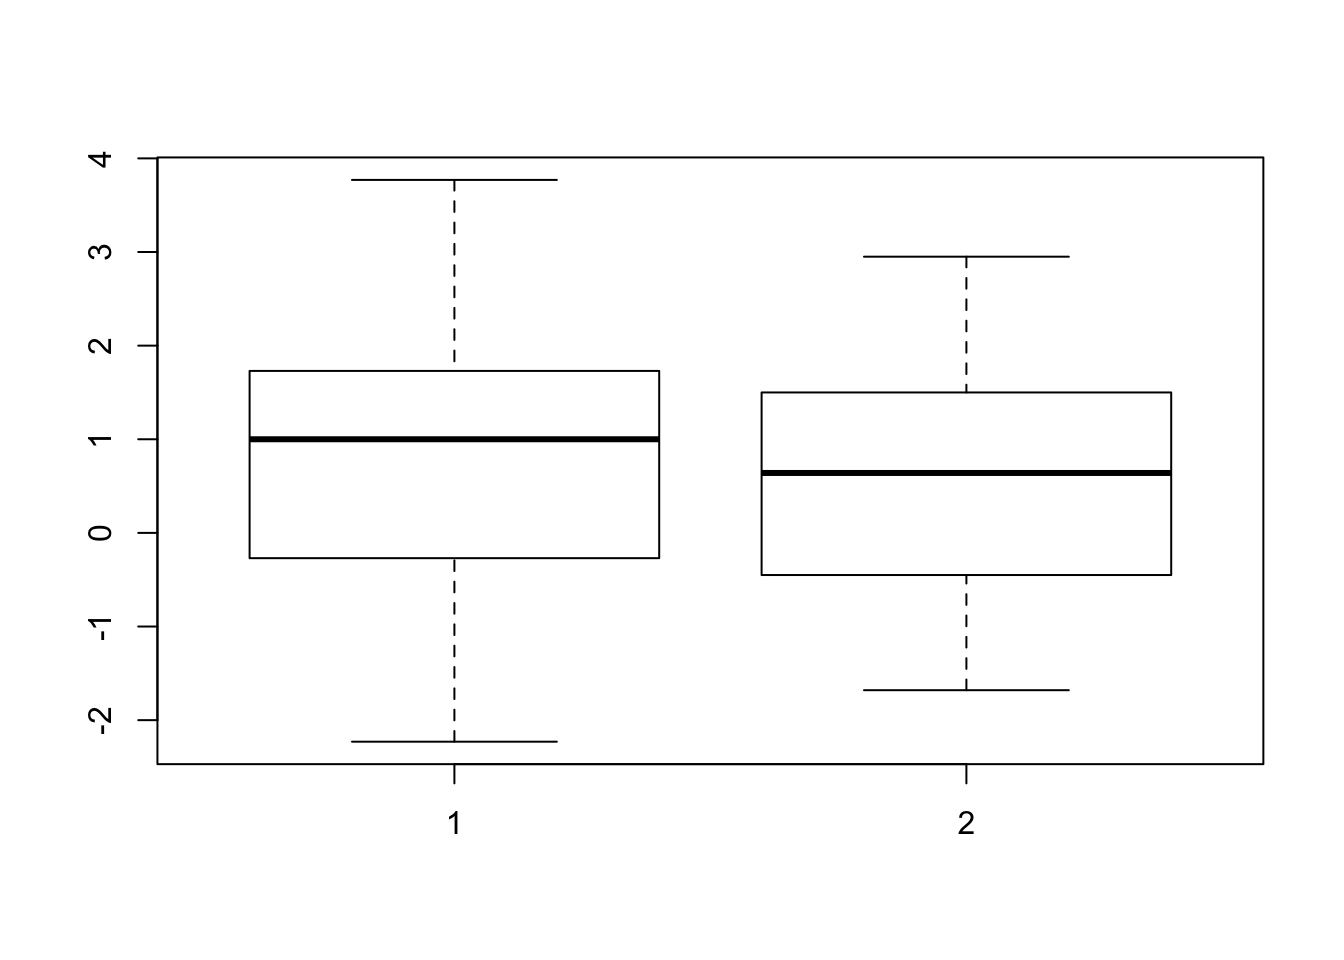
\includegraphics{prfe_files/figure-latex/unnamed-chunk-35-1.pdf}

We can add axis labels and a title to the graph:

\begin{Shaded}
\begin{Highlighting}[]
\KeywordTok{boxplot}\NormalTok{(WT }\OperatorTok{~}\StringTok{ }\NormalTok{LIFE,}
        \DataTypeTok{xlab =} \StringTok{"Life"}\NormalTok{,}
        \DataTypeTok{ylab =} \StringTok{"Weight"}\NormalTok{,}
        \DataTypeTok{main =} \StringTok{"Weight BY Life"}\NormalTok{)}
\end{Highlighting}
\end{Shaded}

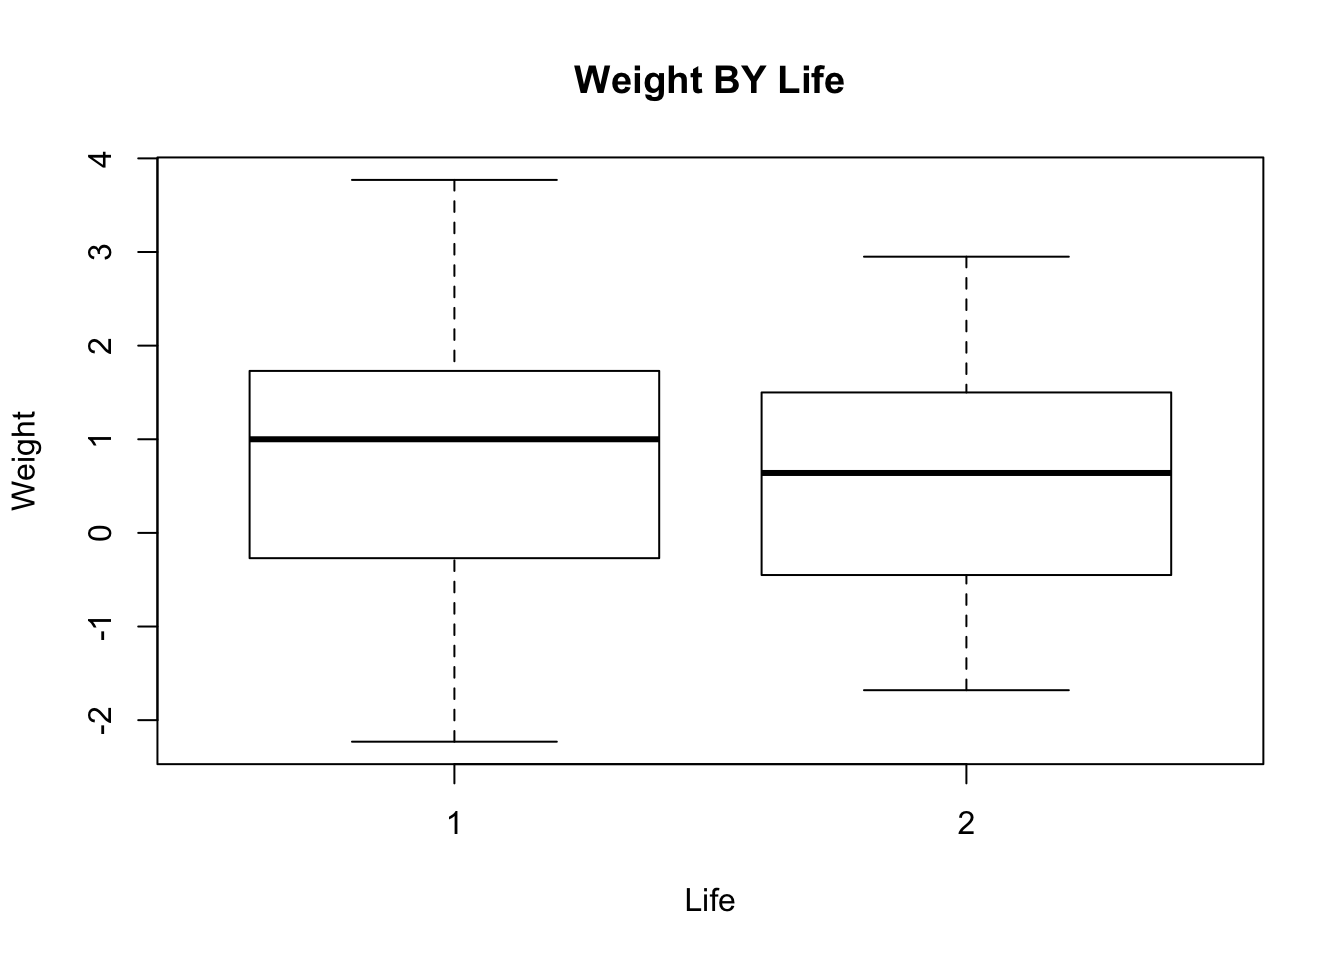
\includegraphics{prfe_files/figure-latex/unnamed-chunk-36-1.pdf}

A more descriptive title might be ``Weight Change BY Considered
Suicide''.

The groups do not seem to differ much in their medians and the
distributions appear to be reasonably symmetrical about their medians
with a similar spread of values.

We can look at the distribution as histograms:

\begin{Shaded}
\begin{Highlighting}[]
\KeywordTok{hist}\NormalTok{(WT[LIFE }\OperatorTok{==}\StringTok{ }\DecValTok{1}\NormalTok{])}
\end{Highlighting}
\end{Shaded}

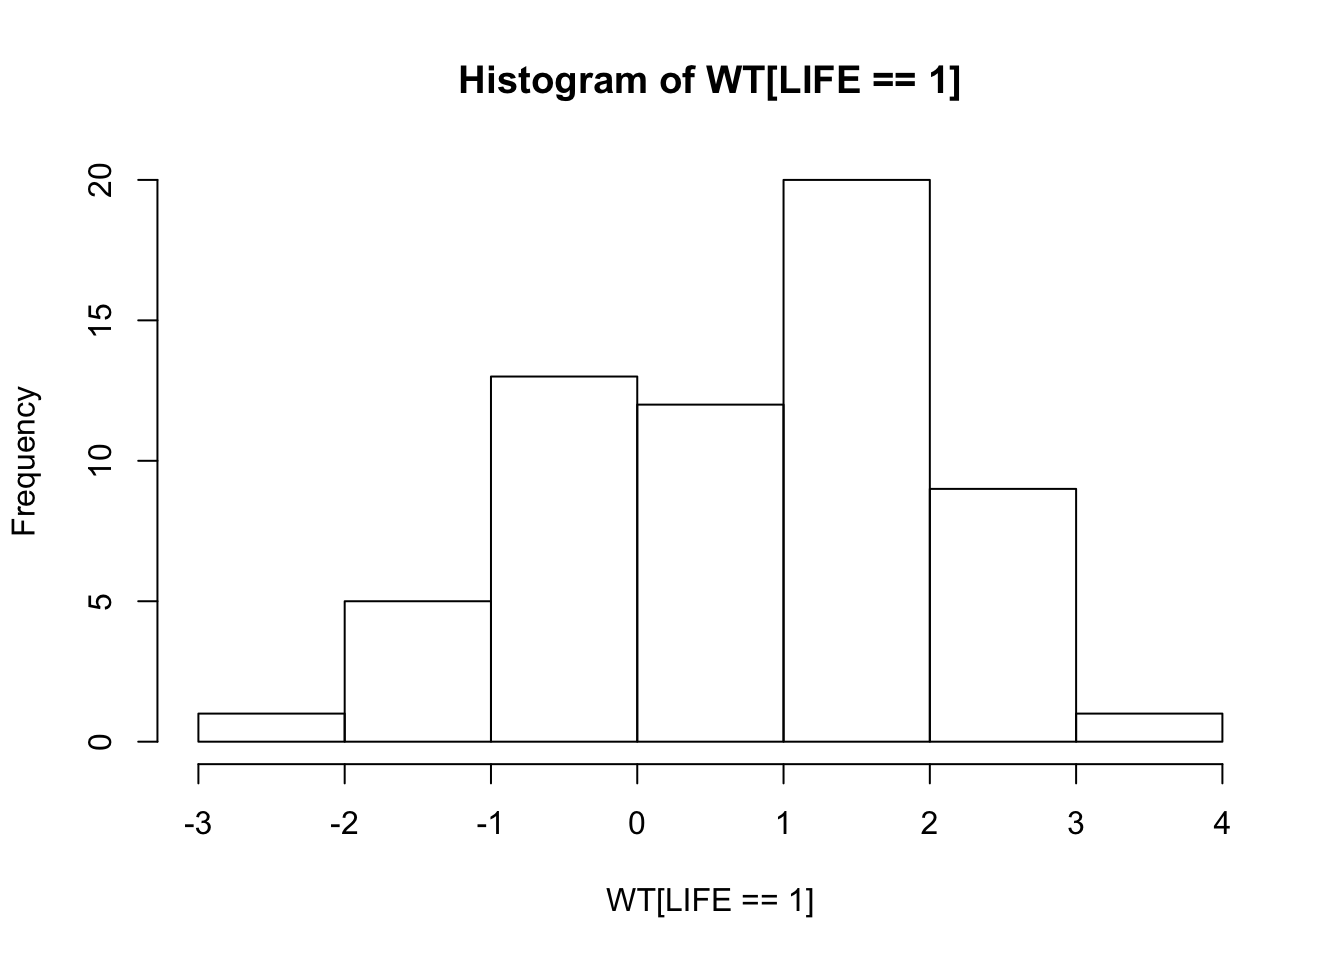
\includegraphics{prfe_files/figure-latex/unnamed-chunk-37-1.pdf}

\begin{Shaded}
\begin{Highlighting}[]
\KeywordTok{hist}\NormalTok{(WT[LIFE }\OperatorTok{==}\StringTok{ }\DecValTok{2}\NormalTok{])}
\end{Highlighting}
\end{Shaded}

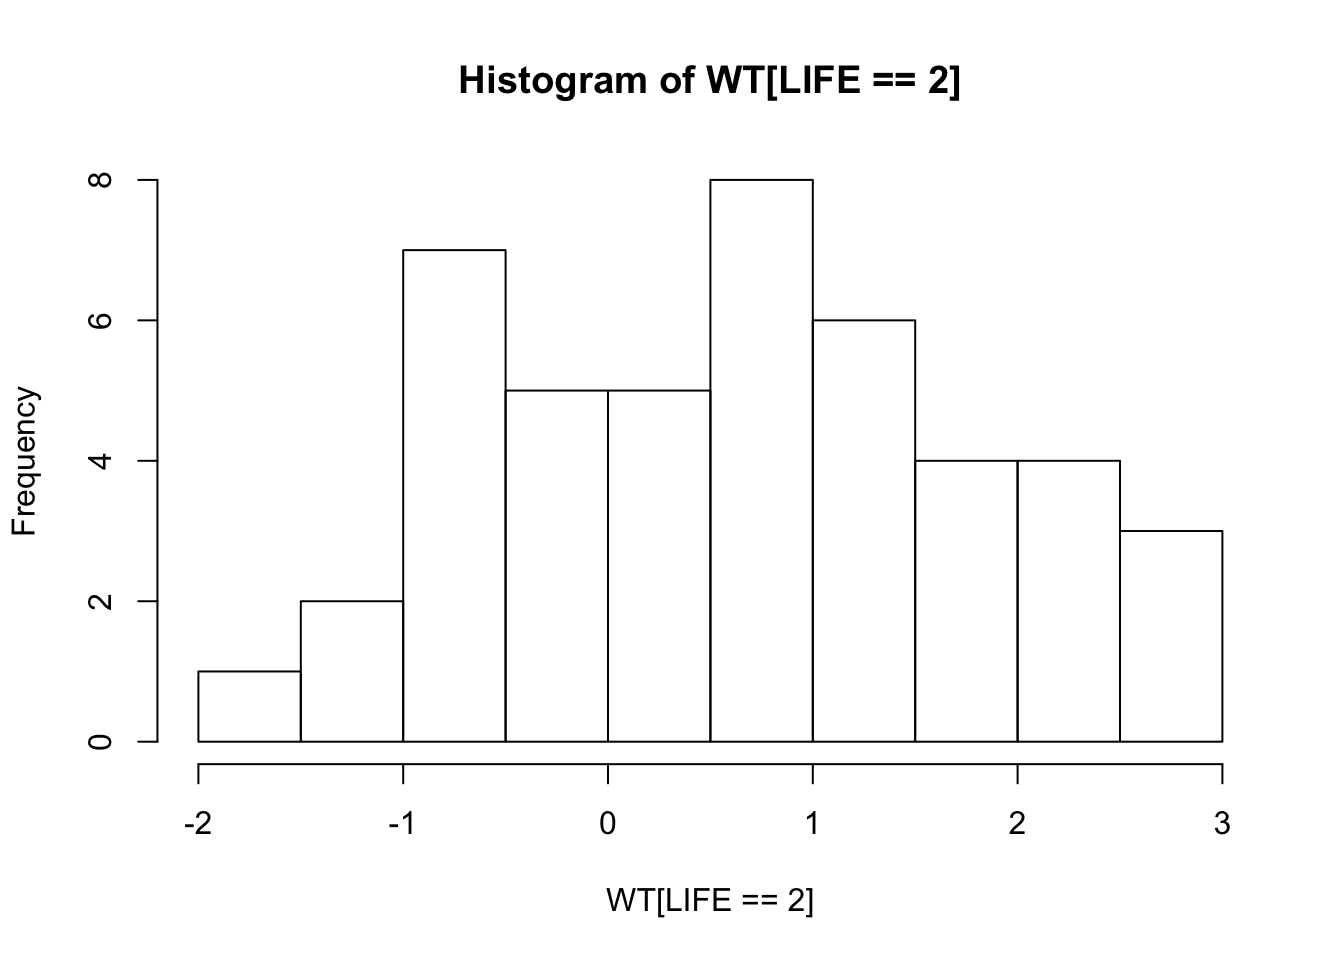
\includegraphics{prfe_files/figure-latex/unnamed-chunk-38-1.pdf}

and check the assumption of normality using quantile-quantile plots:

\begin{Shaded}
\begin{Highlighting}[]
\KeywordTok{qqnorm}\NormalTok{(WT[LIFE }\OperatorTok{==}\StringTok{ }\DecValTok{1}\NormalTok{])}
\KeywordTok{qqline}\NormalTok{(WT[LIFE }\OperatorTok{==}\StringTok{ }\DecValTok{1}\NormalTok{])}
\end{Highlighting}
\end{Shaded}

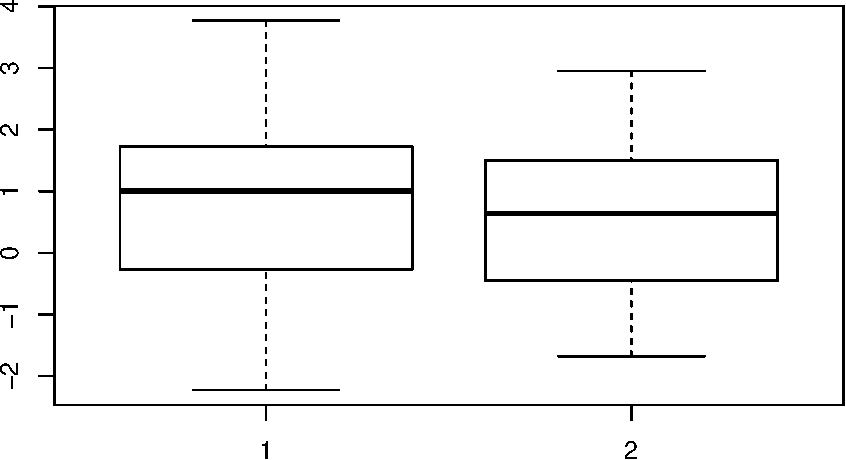
\includegraphics{prfe_files/figure-latex/unnamed-chunk-39-1.pdf}

\begin{Shaded}
\begin{Highlighting}[]
\KeywordTok{qqnorm}\NormalTok{(WT[LIFE }\OperatorTok{==}\StringTok{ }\DecValTok{2}\NormalTok{])}
\KeywordTok{qqline}\NormalTok{(WT[LIFE }\OperatorTok{==}\StringTok{ }\DecValTok{2}\NormalTok{])}
\end{Highlighting}
\end{Shaded}

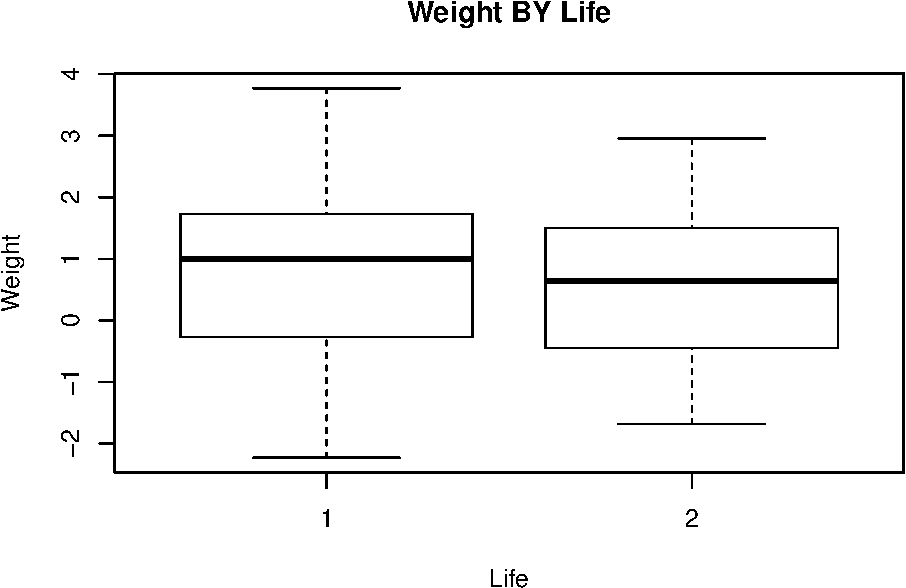
\includegraphics{prfe_files/figure-latex/unnamed-chunk-40-1.pdf}

or by using a formal test:

\begin{Shaded}
\begin{Highlighting}[]
\KeywordTok{shapiro.test}\NormalTok{(WT[LIFE }\OperatorTok{==}\StringTok{ }\DecValTok{1}\NormalTok{])}
\end{Highlighting}
\end{Shaded}

\begin{verbatim}
## 
##  Shapiro-Wilk normality test
## 
## data:  WT[LIFE == 1]
## W = 0.98038, p-value = 0.4336
\end{verbatim}

\begin{Shaded}
\begin{Highlighting}[]
\KeywordTok{shapiro.test}\NormalTok{(WT[LIFE }\OperatorTok{==}\StringTok{ }\DecValTok{2}\NormalTok{])}
\end{Highlighting}
\end{Shaded}

\begin{verbatim}
## 
##  Shapiro-Wilk normality test
## 
## data:  WT[LIFE == 2]
## W = 0.97155, p-value = 0.3292
\end{verbatim}

Remember that we can use the \texttt{by()} function to apply a function
to a data.frame, including statistical functions such as
\texttt{shapiro.test()}:

\begin{Shaded}
\begin{Highlighting}[]
\KeywordTok{by}\NormalTok{(WT, LIFE, shapiro.test)}
\end{Highlighting}
\end{Shaded}

\begin{verbatim}
## LIFE: 1
## 
##  Shapiro-Wilk normality test
## 
## data:  dd[x, ]
## W = 0.98038, p-value = 0.4336
## 
## -------------------------------------------------------- 
## LIFE: 2
## 
##  Shapiro-Wilk normality test
## 
## data:  dd[x, ]
## W = 0.97155, p-value = 0.3292
\end{verbatim}

We can also test whether the variances differ significantly using
\emph{Bartlett's test} for the homogeneity of variances:

\begin{Shaded}
\begin{Highlighting}[]
\KeywordTok{bartlett.test}\NormalTok{(WT, LIFE)}
\end{Highlighting}
\end{Shaded}

\begin{verbatim}
## 
##  Bartlett test of homogeneity of variances
## 
## data:  WT and LIFE
## Bartlett's K-squared = 0.32408, df = 1, p-value = 0.5692
\end{verbatim}

There is no significant difference between the two variances.

Many functions in \texttt{R} have a \emph{formula interface} that may be
used to specify multiple variables and the relations between multiple
variables. We could have used the formula interface with the
\texttt{bartlett.test()} function:

\begin{Shaded}
\begin{Highlighting}[]
\KeywordTok{bartlett.test}\NormalTok{(WT }\OperatorTok{~}\StringTok{ }\NormalTok{LIFE)}
\end{Highlighting}
\end{Shaded}

\begin{verbatim}
## 
##  Bartlett test of homogeneity of variances
## 
## data:  WT by LIFE
## Bartlett's K-squared = 0.32408, df = 1, p-value = 0.5692
\end{verbatim}

Having checked the normality and homogeneity of variance assumptions we
can proceed to carry out a \texttt{t-test}:

\begin{Shaded}
\begin{Highlighting}[]
\KeywordTok{t.test}\NormalTok{(WT }\OperatorTok{~}\StringTok{ }\NormalTok{LIFE, }\DataTypeTok{var.equal =} \OtherTok{TRUE}\NormalTok{)}
\end{Highlighting}
\end{Shaded}

\begin{verbatim}
## 
##  Two Sample t-test
## 
## data:  WT by LIFE
## t = 0.59869, df = 104, p-value = 0.5507
## alternative hypothesis: true difference in means is not equal to 0
## 95 percent confidence interval:
##  -0.3382365  0.6307902
## sample estimates:
## mean in group 1 mean in group 2 
##       0.7867213       0.6404444
\end{verbatim}

There is no evidence that the two groups differ in weight change in the
previous six months.

We could still have performed a \texttt{t-test} if the variances were
not homogenous by setting the \textbf{var.equal} parameter of the
\texttt{t.test()} function to \textbf{FALSE}:

\begin{Shaded}
\begin{Highlighting}[]
\KeywordTok{t.test}\NormalTok{(WT }\OperatorTok{~}\StringTok{ }\NormalTok{LIFE, }\DataTypeTok{var.equal =} \OtherTok{FALSE}\NormalTok{)}
\end{Highlighting}
\end{Shaded}

\begin{verbatim}
## 
##  Welch Two Sample t-test
## 
## data:  WT by LIFE
## t = 0.60608, df = 98.866, p-value = 0.5459
## alternative hypothesis: true difference in means is not equal to 0
## 95 percent confidence interval:
##  -0.3326225  0.6251763
## sample estimates:
## mean in group 1 mean in group 2 
##       0.7867213       0.6404444
\end{verbatim}

or performed a non-parametric test:

\begin{Shaded}
\begin{Highlighting}[]
\KeywordTok{wilcox.test}\NormalTok{(WT }\OperatorTok{~}\StringTok{ }\NormalTok{LIFE)}
\end{Highlighting}
\end{Shaded}

\begin{verbatim}
## 
##  Wilcoxon rank sum test with continuity correction
## 
## data:  WT by LIFE
## W = 1488, p-value = 0.4622
## alternative hypothesis: true location shift is not equal to 0
\end{verbatim}

An alternative, and more general, non-parametric test is:

\begin{Shaded}
\begin{Highlighting}[]
\KeywordTok{kruskal.test}\NormalTok{(WT }\OperatorTok{~}\StringTok{ }\NormalTok{LIFE)}
\end{Highlighting}
\end{Shaded}

\begin{verbatim}
## 
##  Kruskal-Wallis rank sum test
## 
## data:  WT by LIFE
## Kruskal-Wallis chi-squared = 0.54521, df = 1, p-value = 0.4603
\end{verbatim}

We can use the \texttt{table()} function to examine the differences in
depression between the two groups:

\begin{Shaded}
\begin{Highlighting}[]
\KeywordTok{table}\NormalTok{(DEP, LIFE)}
\end{Highlighting}
\end{Shaded}

\begin{verbatim}
##    LIFE
## DEP  1  2
##   1  0 26
##   2 42 24
##   3 16  1
\end{verbatim}

The two distributions look very different from each other. We can test
this using a chi-square test on the table:

\begin{Shaded}
\begin{Highlighting}[]
\KeywordTok{chisq.test}\NormalTok{(}\KeywordTok{table}\NormalTok{(DEP, LIFE))}
\end{Highlighting}
\end{Shaded}

\begin{verbatim}
## 
##  Pearson's Chi-squared test
## 
## data:  table(DEP, LIFE)
## X-squared = 43.876, df = 2, p-value = 2.968e-10
\end{verbatim}

Note that we passed the output of the \texttt{table()} function directly
to the \texttt{chisq.test()} function. We could have saved the table as
an object first and then passed the object to the \texttt{chisq.test()}
function:

\begin{Shaded}
\begin{Highlighting}[]
\NormalTok{tab <-}\StringTok{ }\KeywordTok{table}\NormalTok{(DEP, LIFE)}
\KeywordTok{chisq.test}\NormalTok{(tab)}
\end{Highlighting}
\end{Shaded}

\begin{verbatim}
## 
##  Pearson's Chi-squared test
## 
## data:  tab
## X-squared = 43.876, df = 2, p-value = 2.968e-10
\end{verbatim}

The \texttt{tab} object contains the output of the \texttt{table()}
function:

\begin{Shaded}
\begin{Highlighting}[]
\KeywordTok{class}\NormalTok{(tab)}
\end{Highlighting}
\end{Shaded}

\begin{verbatim}
## [1] "table"
\end{verbatim}

\begin{Shaded}
\begin{Highlighting}[]
\NormalTok{tab}
\end{Highlighting}
\end{Shaded}

\begin{verbatim}
##    LIFE
## DEP  1  2
##   1  0 26
##   2 42 24
##   3 16  1
\end{verbatim}

We can pass this table object to another function. For example:

\begin{Shaded}
\begin{Highlighting}[]
\KeywordTok{fisher.test}\NormalTok{(tab)}
\end{Highlighting}
\end{Shaded}

\begin{verbatim}
## 
##  Fisher's Exact Test for Count Data
## 
## data:  tab
## p-value = 1.316e-12
## alternative hypothesis: two.sided
\end{verbatim}

When we are finished with the tab object we can delete it using the
\texttt{rm()} function:

\begin{Shaded}
\begin{Highlighting}[]
\KeywordTok{rm}\NormalTok{(tab)}
\end{Highlighting}
\end{Shaded}

You can see a list of available objects using the \texttt{ls()}
function:

\begin{Shaded}
\begin{Highlighting}[]
\KeywordTok{ls}\NormalTok{()}
\end{Highlighting}
\end{Shaded}

\begin{verbatim}
## [1] "fem"
\end{verbatim}

This should just show the \texttt{fem} object.

We can examine the association between loss of interest in sex and
considering suicide in the same way:

\begin{Shaded}
\begin{Highlighting}[]
\NormalTok{tab <-}\StringTok{ }\KeywordTok{table}\NormalTok{(SEX, LIFE)}
\NormalTok{tab}
\end{Highlighting}
\end{Shaded}

\begin{verbatim}
##    LIFE
## SEX  1  2
##   1 58 38
##   2  5 12
\end{verbatim}

\begin{Shaded}
\begin{Highlighting}[]
\KeywordTok{fisher.test}\NormalTok{(tab)}
\end{Highlighting}
\end{Shaded}

\begin{verbatim}
## 
##  Fisher's Exact Test for Count Data
## 
## data:  tab
## p-value = 0.03175
## alternative hypothesis: true odds ratio is not equal to 1
## 95 percent confidence interval:
##   1.080298 14.214482
## sample estimates:
## odds ratio 
##   3.620646
\end{verbatim}

Note that with a two-by-two table the \texttt{fisher.test()} function
produces an estimate of, and confidence intervals for, the odds ratio.
Again, we will delete the \texttt{tab} object:

\begin{Shaded}
\begin{Highlighting}[]
\KeywordTok{rm}\NormalTok{(tab)}
\end{Highlighting}
\end{Shaded}

We could have performed the Fisher exact test without creating the tab
object by passing the output of the \texttt{table()} function directly
to the \texttt{fisher.test()} function:

\begin{Shaded}
\begin{Highlighting}[]
\KeywordTok{fisher.test}\NormalTok{(}\KeywordTok{table}\NormalTok{(SEX, LIFE))}
\end{Highlighting}
\end{Shaded}

\begin{verbatim}
## 
##  Fisher's Exact Test for Count Data
## 
## data:  table(SEX, LIFE)
## p-value = 0.03175
## alternative hypothesis: true odds ratio is not equal to 1
## 95 percent confidence interval:
##   1.080298 14.214482
## sample estimates:
## odds ratio 
##   3.620646
\end{verbatim}

Choose whichever method you find easiest but remember that it is easy to
save the results of any function for later use.

We can explore the correlation between two variables using the
\texttt{cor()} function:

\begin{Shaded}
\begin{Highlighting}[]
\KeywordTok{cor}\NormalTok{(IQ, WT, }\DataTypeTok{use =} \StringTok{"pairwise.complete.obs"}\NormalTok{)}
\end{Highlighting}
\end{Shaded}

\begin{verbatim}
## [1] -0.2917158
\end{verbatim}

or by using a scatter plot:

\begin{Shaded}
\begin{Highlighting}[]
\KeywordTok{plot}\NormalTok{(IQ, WT)}
\end{Highlighting}
\end{Shaded}

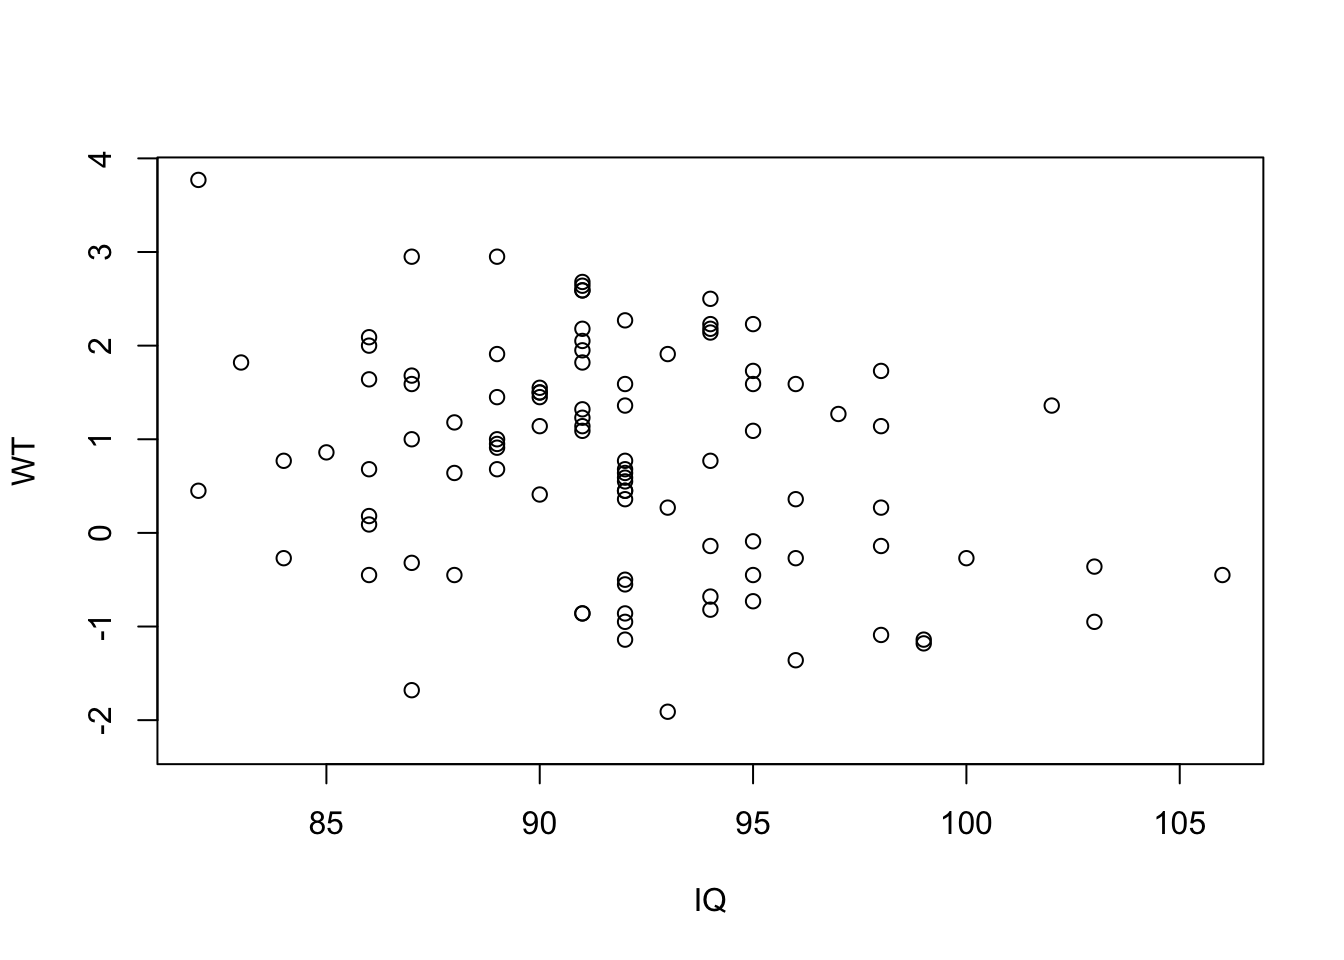
\includegraphics{prfe_files/figure-latex/unnamed-chunk-60-1.pdf}

and by a formal test:

\begin{Shaded}
\begin{Highlighting}[]
\KeywordTok{cor.test}\NormalTok{(IQ, WT)}
\end{Highlighting}
\end{Shaded}

\begin{verbatim}
## 
##  Pearson's product-moment correlation
## 
## data:  IQ and WT
## t = -3.0192, df = 98, p-value = 0.003231
## alternative hypothesis: true correlation is not equal to 0
## 95 percent confidence interval:
##  -0.4616804 -0.1010899
## sample estimates:
##        cor 
## -0.2917158
\end{verbatim}

With some functions you can pass an entire data.frame rather than a list
of variables:

\begin{Shaded}
\begin{Highlighting}[]
\KeywordTok{cor}\NormalTok{(fem, }\DataTypeTok{use =} \StringTok{"pairwise.complete.obs"}\NormalTok{)}
\end{Highlighting}
\end{Shaded}

\begin{verbatim}
##               ID         AGE            IQ         ANX           DEP
## ID    1.00000000  0.03069077  0.0370598672 -0.02941825 -0.0554147209
## AGE   0.03069077  1.00000000 -0.4345435680  0.06734300 -0.0387049246
## IQ    0.03705987 -0.43454357  1.0000000000 -0.02323787 -0.0001307404
## ANX  -0.02941825  0.06734300 -0.0232378691  1.00000000  0.5437946347
## DEP  -0.05541472 -0.03870492 -0.0001307404  0.54379463  1.0000000000
## SLP  -0.07268743  0.02606547  0.0812993104  0.22317875  0.5248724551
## SEX   0.08999634  0.10609216 -0.0536558660 -0.21062493 -0.3058422258
## LIFE -0.05604349 -0.10300193 -0.0915396469 -0.34211268 -0.6139017253
## WT    0.02640131  0.41574411 -0.2917157832  0.11817532  0.0233742465
##               SLP         SEX        LIFE           WT
## ID   -0.072687434  0.08999634 -0.05604349  0.026401310
## AGE   0.026065468  0.10609216 -0.10300193  0.415744109
## IQ    0.081299310 -0.05365587 -0.09153965 -0.291715783
## ANX   0.223178752 -0.21062493 -0.34211268  0.118175321
## DEP   0.524872455 -0.30584223 -0.61390173  0.023374247
## SLP   1.000000000 -0.29053971 -0.35186578 -0.009259774
## SEX  -0.290539709  1.00000000  0.22316967 -0.027826514
## LIFE -0.351865775  0.22316967  1.00000000 -0.058605326
## WT   -0.009259774 -0.02782651 -0.05860533  1.000000000
\end{verbatim}

\begin{Shaded}
\begin{Highlighting}[]
\KeywordTok{pairs}\NormalTok{(fem)}
\end{Highlighting}
\end{Shaded}

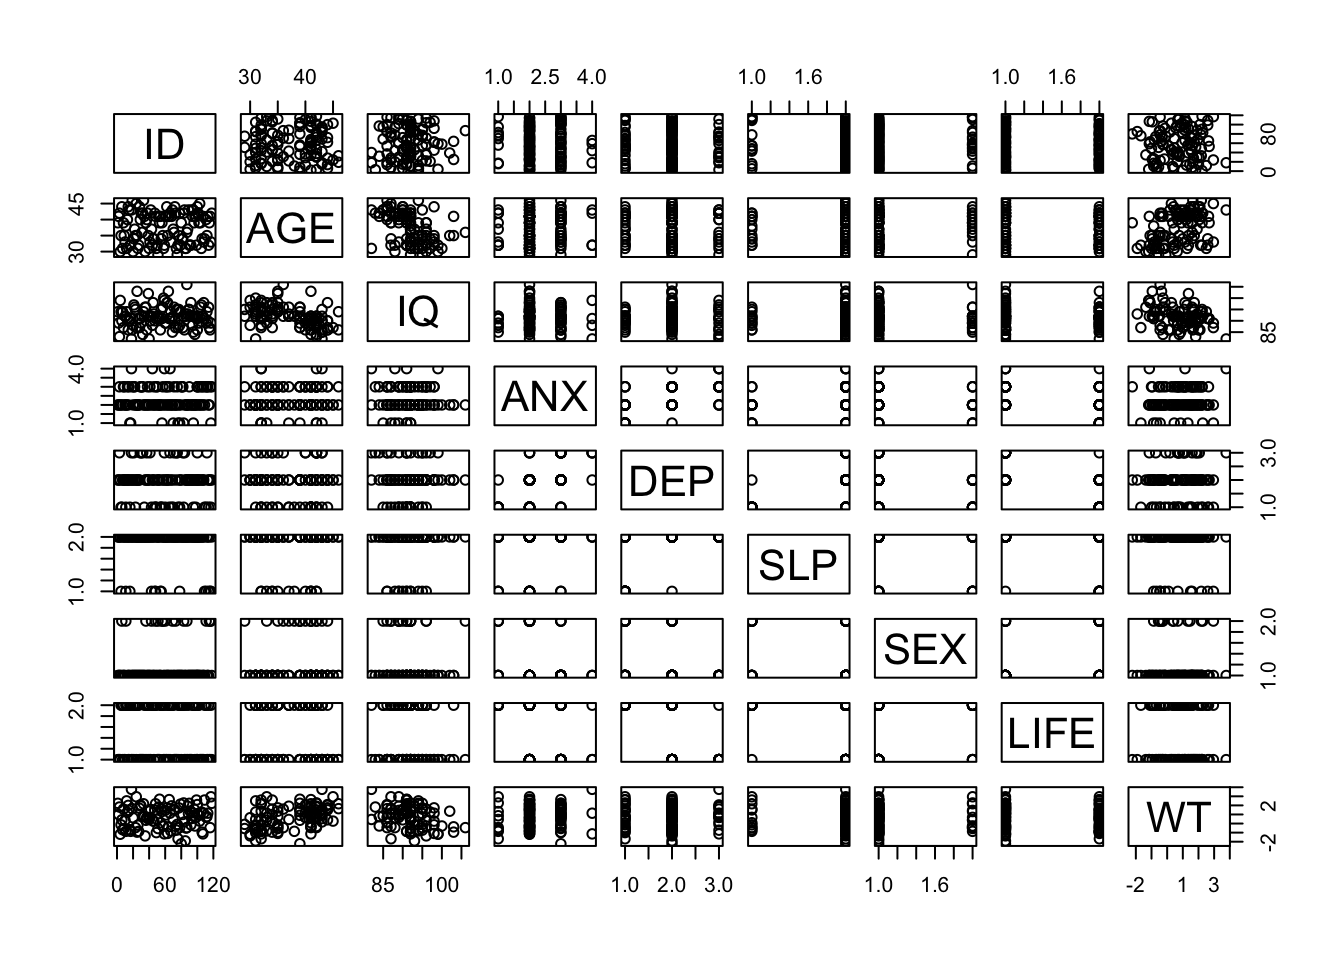
\includegraphics{prfe_files/figure-latex/unnamed-chunk-62-1.pdf}

The output can be a little confusing particularly if it includes
categorical or record identifying variables. To avoid this we can create
a new object that contains only the columns we are interested in using
the column binding \texttt{cbind()} function:

\begin{Shaded}
\begin{Highlighting}[]
\NormalTok{newfem <-}\StringTok{ }\KeywordTok{cbind}\NormalTok{(AGE, IQ, WT)}
\KeywordTok{cor}\NormalTok{(newfem, }\DataTypeTok{use =} \StringTok{"pairwise.complete.obs"}\NormalTok{)}
\end{Highlighting}
\end{Shaded}

\begin{verbatim}
##            AGE         IQ         WT
## AGE  1.0000000 -0.4345436  0.4157441
## IQ  -0.4345436  1.0000000 -0.2917158
## WT   0.4157441 -0.2917158  1.0000000
\end{verbatim}

\begin{Shaded}
\begin{Highlighting}[]
\KeywordTok{pairs}\NormalTok{(newfem)}
\end{Highlighting}
\end{Shaded}

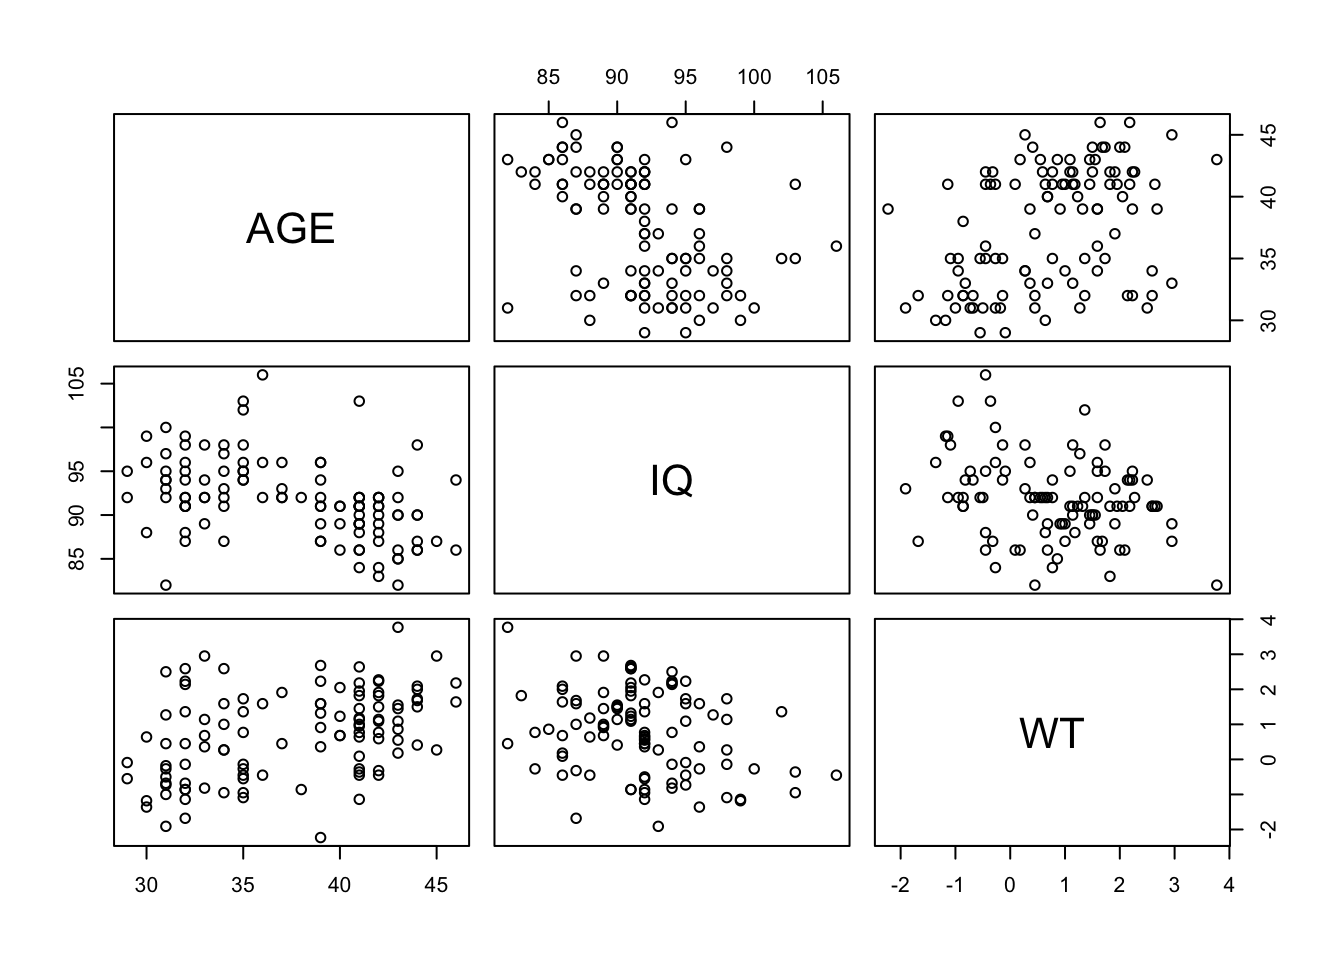
\includegraphics{prfe_files/figure-latex/unnamed-chunk-63-1.pdf}

When we have finished with the \texttt{newfem} object we can delete it:

\begin{Shaded}
\begin{Highlighting}[]
\KeywordTok{rm}\NormalTok{(newfem)}
\end{Highlighting}
\end{Shaded}

There was no real need to create the \texttt{newfem} object as we could
have fed the output of the \texttt{cbind()} function directly to the
\texttt{cor()} or \texttt{pairs()} function:

\begin{Shaded}
\begin{Highlighting}[]
\KeywordTok{cor}\NormalTok{(}\KeywordTok{cbind}\NormalTok{(AGE, IQ, WT), }\DataTypeTok{use =} \StringTok{"pairwise.complete.obs"}\NormalTok{)}
\end{Highlighting}
\end{Shaded}

\begin{verbatim}
##            AGE         IQ         WT
## AGE  1.0000000 -0.4345436  0.4157441
## IQ  -0.4345436  1.0000000 -0.2917158
## WT   0.4157441 -0.2917158  1.0000000
\end{verbatim}

\begin{Shaded}
\begin{Highlighting}[]
\KeywordTok{pairs}\NormalTok{(}\KeywordTok{cbind}\NormalTok{(AGE, IQ, WT))}
\end{Highlighting}
\end{Shaded}

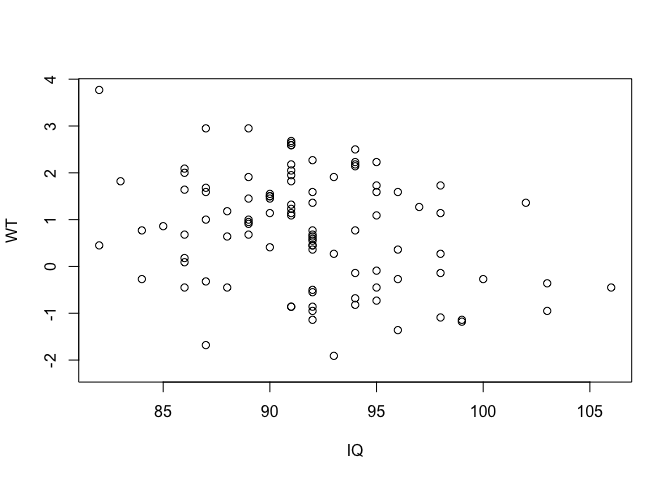
\includegraphics{prfe_files/figure-latex/unnamed-chunk-65-1.pdf}

It is, however, easier to work with the \texttt{newfem} object rather
than having to retype the \texttt{cbind()} function. This is
particularly true if you wanted to continue with an analysis of just the
three variables.

The relationship between \texttt{AGE} and \texttt{WT} can be plotted
using the \texttt{plot()} function:

\begin{Shaded}
\begin{Highlighting}[]
\KeywordTok{plot}\NormalTok{(AGE, WT)}
\end{Highlighting}
\end{Shaded}

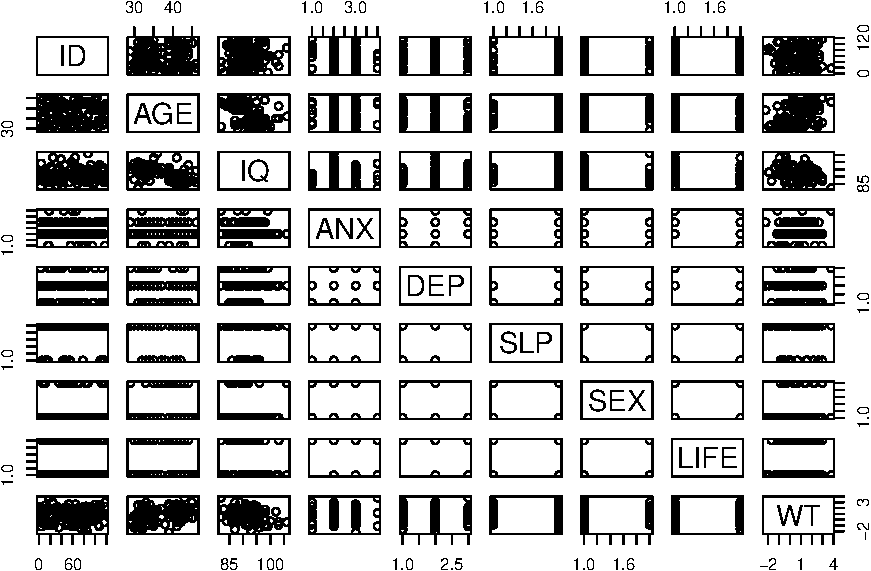
\includegraphics{prfe_files/figure-latex/unnamed-chunk-66-1.pdf}

And tested using the \texttt{cor()} and \texttt{cor.test()} functions:

\begin{Shaded}
\begin{Highlighting}[]
\KeywordTok{cor}\NormalTok{(AGE, WT, }\DataTypeTok{use =} \StringTok{"pairwise.complete.obs"}\NormalTok{)}
\end{Highlighting}
\end{Shaded}

\begin{verbatim}
## [1] 0.4157441
\end{verbatim}

\begin{Shaded}
\begin{Highlighting}[]
\KeywordTok{cor.test}\NormalTok{(AGE, WT)}
\end{Highlighting}
\end{Shaded}

\begin{verbatim}
## 
##  Pearson's product-moment correlation
## 
## data:  AGE and WT
## t = 4.6841, df = 105, p-value = 8.457e-06
## alternative hypothesis: true correlation is not equal to 0
## 95 percent confidence interval:
##  0.2452434 0.5612979
## sample estimates:
##       cor 
## 0.4157441
\end{verbatim}

Or by using the linear modelling \texttt{lm()} function:

\begin{Shaded}
\begin{Highlighting}[]
\KeywordTok{summary}\NormalTok{(}\KeywordTok{lm}\NormalTok{(WT }\OperatorTok{~}\StringTok{ }\NormalTok{AGE))}
\end{Highlighting}
\end{Shaded}

\begin{verbatim}
## 
## Call:
## lm(formula = WT ~ AGE)
## 
## Residuals:
##      Min       1Q   Median       3Q      Max 
## -3.10678 -0.85922 -0.05453  0.71434  2.70874 
## 
## Coefficients:
##             Estimate Std. Error t value Pr(>|t|)    
## (Intercept) -3.25405    0.85547  -3.804  0.00024 ***
## AGE          0.10592    0.02261   4.684 8.46e-06 ***
## ---
## Signif. codes:  0 '***' 0.001 '**' 0.01 '*' 0.05 '.' 0.1 ' ' 1
## 
## Residual standard error: 1.128 on 105 degrees of freedom
##   (11 observations deleted due to missingness)
## Multiple R-squared:  0.1728, Adjusted R-squared:  0.165 
## F-statistic: 21.94 on 1 and 105 DF,  p-value: 8.457e-06
\end{verbatim}

We use the \texttt{summary()} function here to extract summary
information from the output of the \texttt{lm()} function.

It is often more useful to use \texttt{lm()} to create an object:

\begin{Shaded}
\begin{Highlighting}[]
\NormalTok{fem.lm <-}\StringTok{ }\KeywordTok{lm}\NormalTok{(WT }\OperatorTok{~}\StringTok{ }\NormalTok{AGE)}
\end{Highlighting}
\end{Shaded}

And use the output in other functions:

\begin{Shaded}
\begin{Highlighting}[]
\KeywordTok{summary}\NormalTok{(fem.lm)}
\end{Highlighting}
\end{Shaded}

\begin{verbatim}
## 
## Call:
## lm(formula = WT ~ AGE)
## 
## Residuals:
##      Min       1Q   Median       3Q      Max 
## -3.10678 -0.85922 -0.05453  0.71434  2.70874 
## 
## Coefficients:
##             Estimate Std. Error t value Pr(>|t|)    
## (Intercept) -3.25405    0.85547  -3.804  0.00024 ***
## AGE          0.10592    0.02261   4.684 8.46e-06 ***
## ---
## Signif. codes:  0 '***' 0.001 '**' 0.01 '*' 0.05 '.' 0.1 ' ' 1
## 
## Residual standard error: 1.128 on 105 degrees of freedom
##   (11 observations deleted due to missingness)
## Multiple R-squared:  0.1728, Adjusted R-squared:  0.165 
## F-statistic: 21.94 on 1 and 105 DF,  p-value: 8.457e-06
\end{verbatim}

\begin{Shaded}
\begin{Highlighting}[]
\KeywordTok{plot}\NormalTok{(AGE, WT)}
\KeywordTok{abline}\NormalTok{(fem.lm)}
\end{Highlighting}
\end{Shaded}

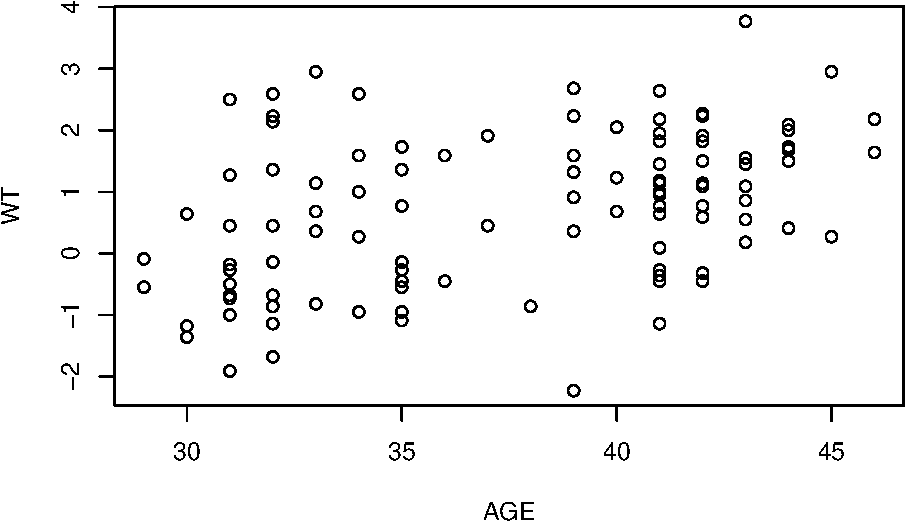
\includegraphics{prfe_files/figure-latex/unnamed-chunk-70-1.pdf}

In this case we are passing the intercept and slope information held in
the \texttt{fem.lm} object to the \texttt{abline()} function which draws
a regression line. The \texttt{abline()} function adds to an existing
plot. This means that you need to keep the scatter plot of \texttt{AGE}
and \texttt{WT} open before issuing the \texttt{abline()} function call.

A useful function to apply to the \texttt{fem.lm} object is
\texttt{plot()} which produces diagnostic plots of the linear model:

\begin{Shaded}
\begin{Highlighting}[]
\KeywordTok{plot}\NormalTok{(fem.lm)}
\end{Highlighting}
\end{Shaded}

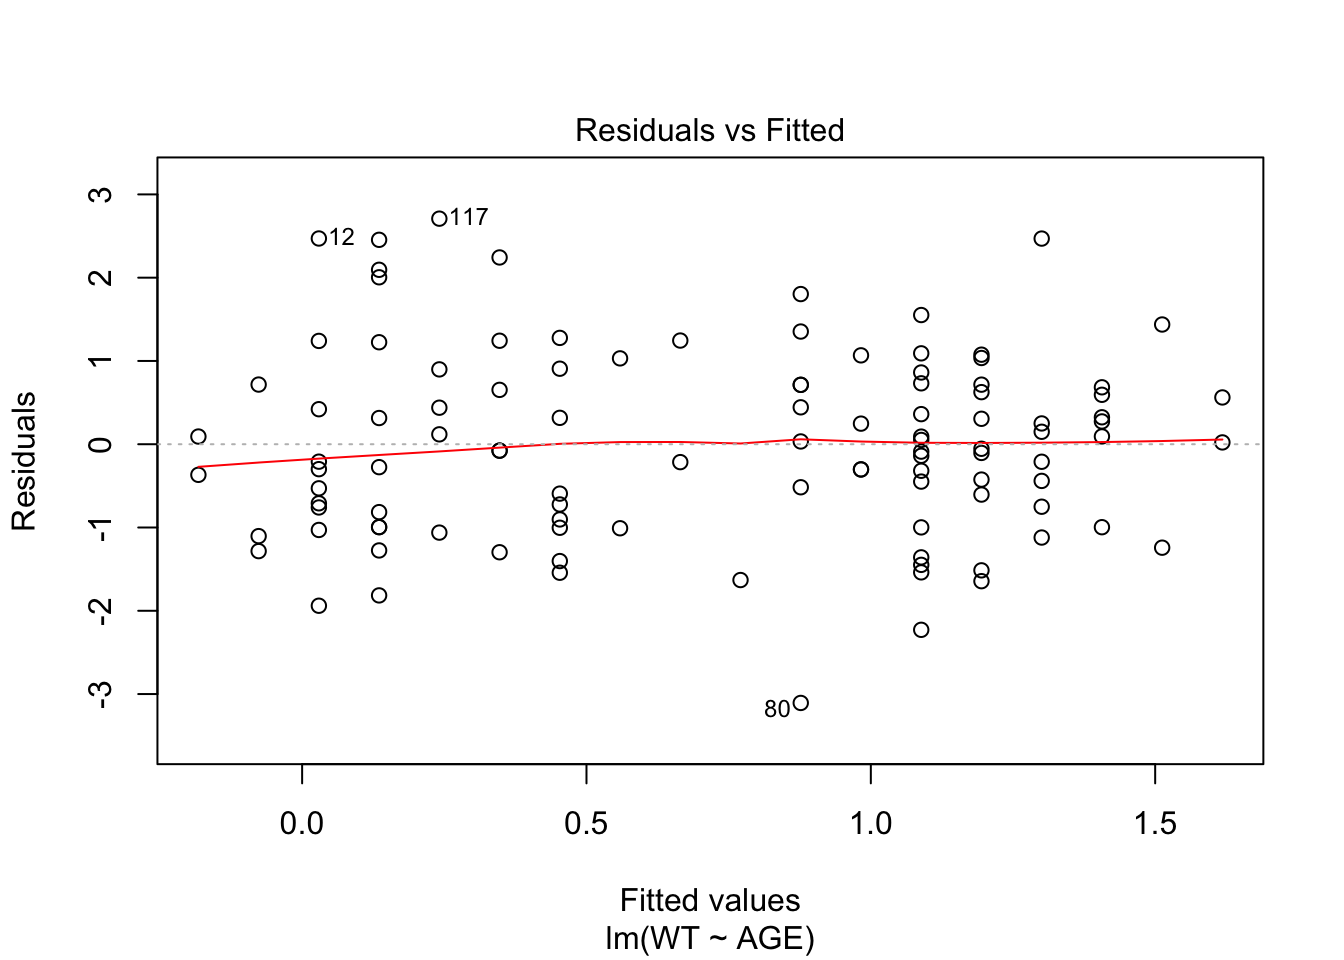
\includegraphics{prfe_files/figure-latex/unnamed-chunk-71-1.pdf}
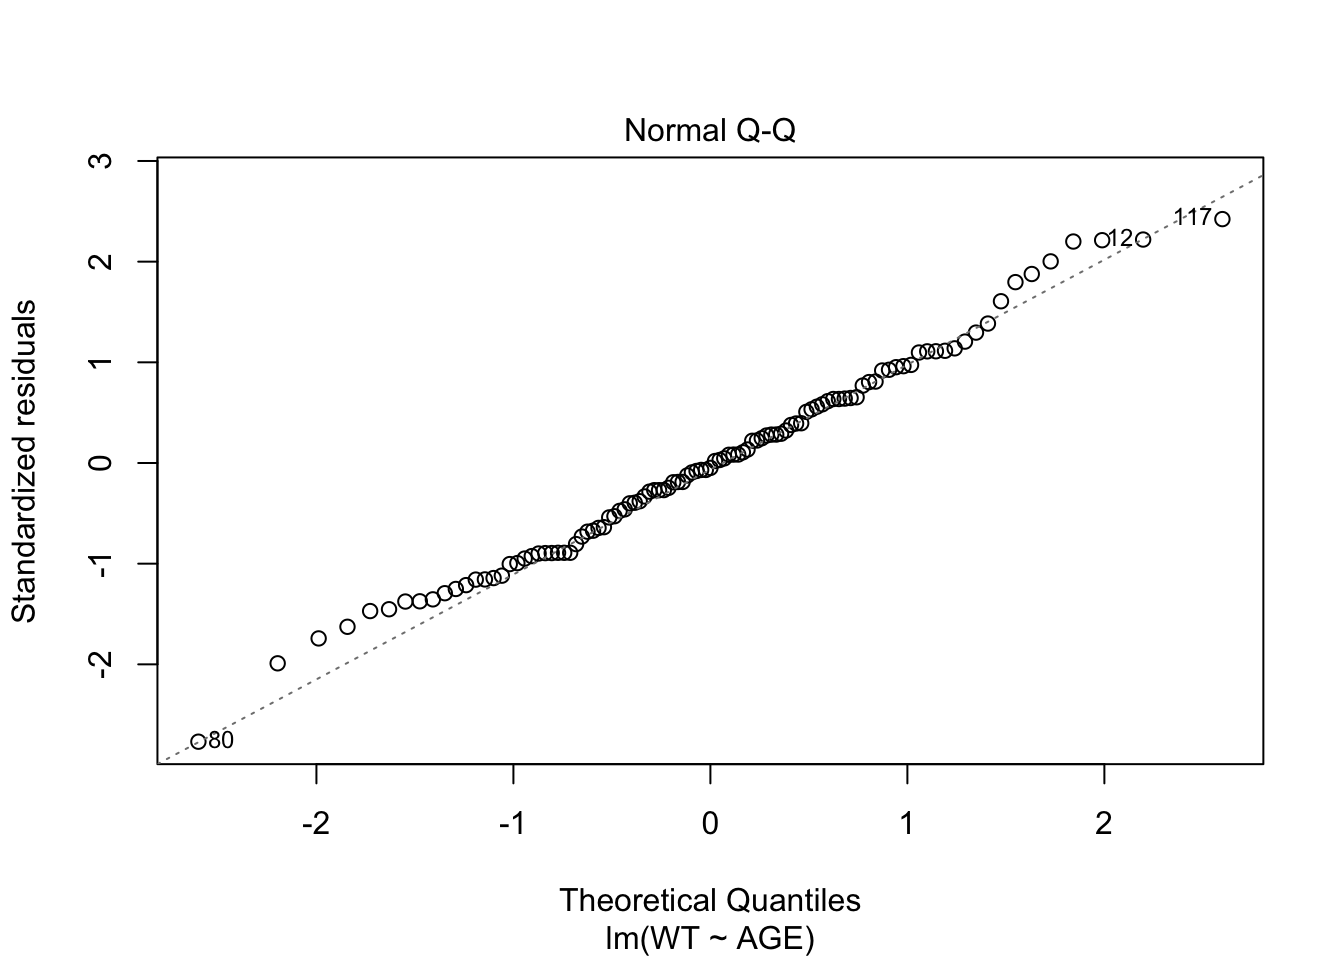
\includegraphics{prfe_files/figure-latex/unnamed-chunk-71-2.pdf}
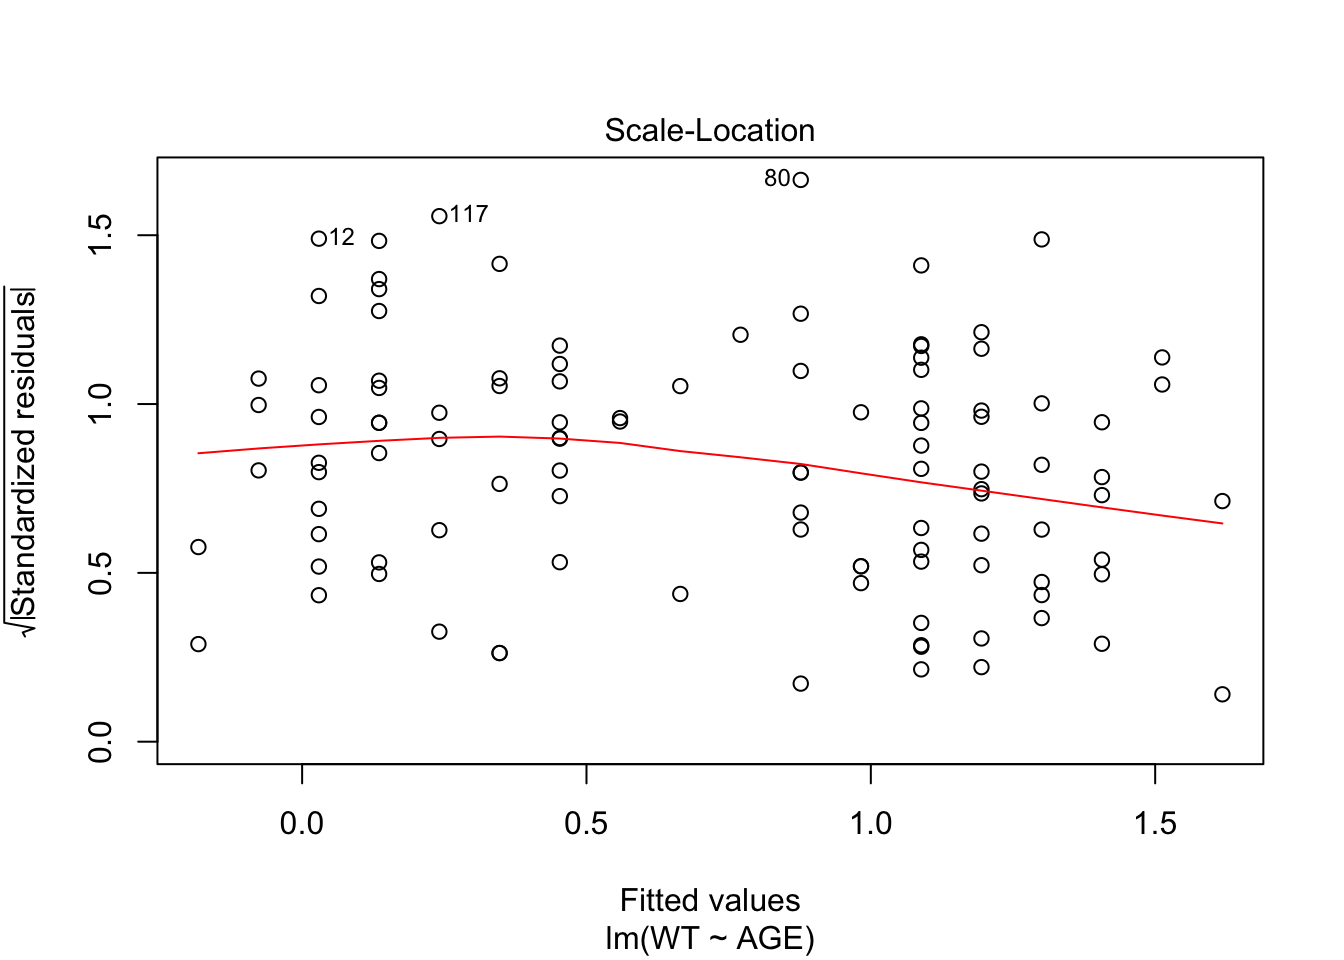
\includegraphics{prfe_files/figure-latex/unnamed-chunk-71-3.pdf}
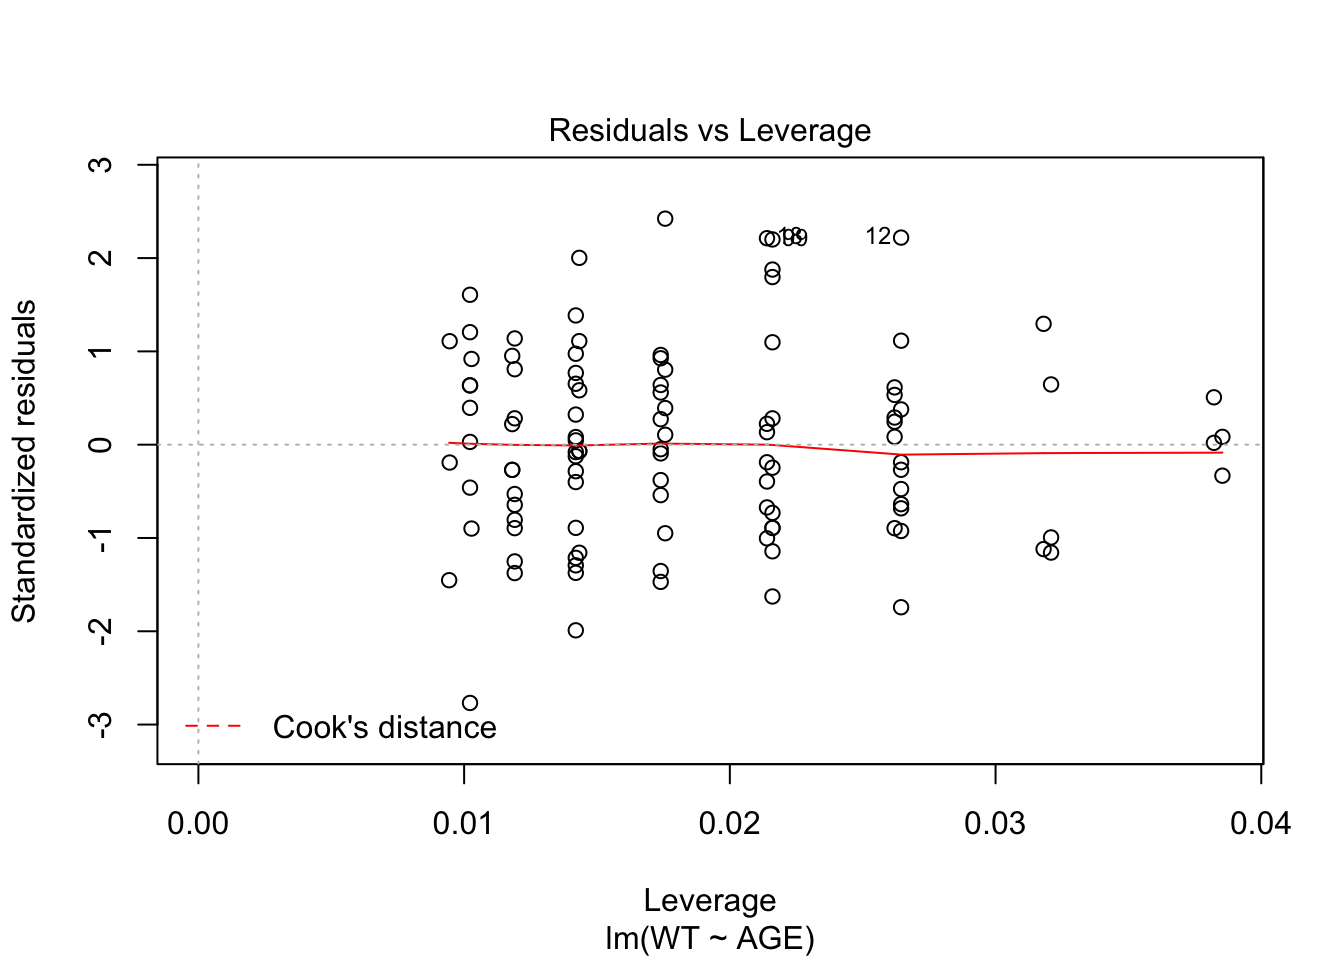
\includegraphics{prfe_files/figure-latex/unnamed-chunk-71-4.pdf}

Objects created by the \texttt{lm()} function (or any of the modelling
functions) can use up a lot of memory so we should remove them when we
no longer need them:

\begin{Shaded}
\begin{Highlighting}[]
\KeywordTok{rm}\NormalTok{(fem.lm)}
\end{Highlighting}
\end{Shaded}

It might be interesting to see whether a similar relationship exists
between \texttt{AGE} and \texttt{WT} for those who have and have not
considered suicide. This can be done using the \texttt{coplot()}
function:

\begin{Shaded}
\begin{Highlighting}[]
\KeywordTok{coplot}\NormalTok{(WT }\OperatorTok{~}\StringTok{ }\NormalTok{AGE }\OperatorTok{|}\StringTok{ }\KeywordTok{as.factor}\NormalTok{(LIFE))}
\end{Highlighting}
\end{Shaded}

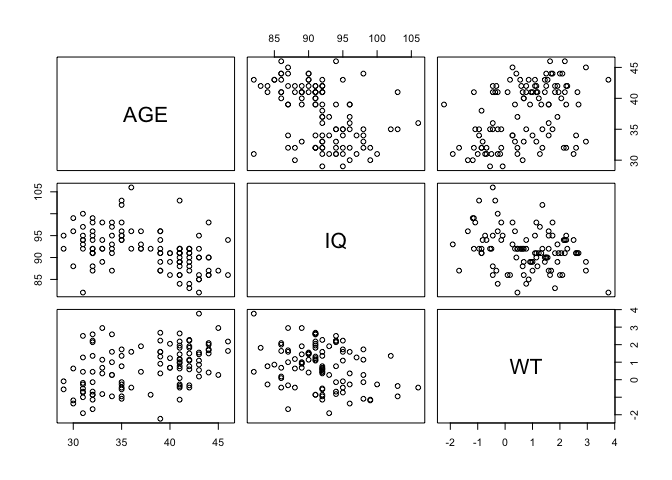
\includegraphics{prfe_files/figure-latex/unnamed-chunk-73-1.pdf}

\begin{verbatim}
## 
##  Missing rows: 21, 22, 31, 43, 44, 45, 69, 81, 101, 104, 114, 115
\end{verbatim}

The two plots looks similar. We could also use \texttt{coplot()} to
investigate the relationship between \texttt{AGE} and \texttt{WT} for
categories of both \texttt{LIFE} and \texttt{SEX}:

\begin{Shaded}
\begin{Highlighting}[]
\KeywordTok{coplot}\NormalTok{(WT }\OperatorTok{~}\StringTok{ }\NormalTok{AGE }\OperatorTok{|}\StringTok{ }\KeywordTok{as.factor}\NormalTok{(LIFE) }\OperatorTok{*}\StringTok{ }\KeywordTok{as.factor}\NormalTok{(SEX))}
\end{Highlighting}
\end{Shaded}

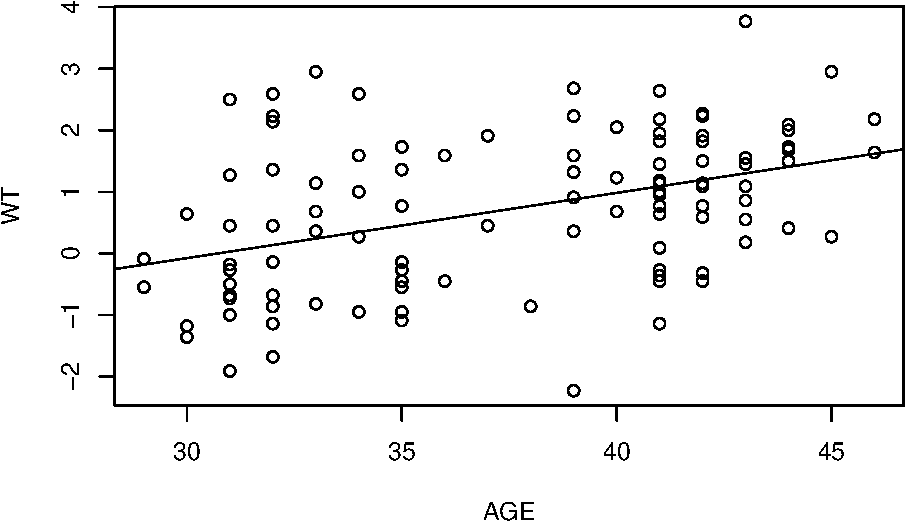
\includegraphics{prfe_files/figure-latex/unnamed-chunk-74-1.pdf}

\begin{verbatim}
## 
##  Missing rows: 12, 17, 21, 22, 31, 43, 44, 45, 66, 69, 81, 101, 104, 105, 114, 115
\end{verbatim}

although the numbers are too small for this to be useful here.

We used the \texttt{as.factor()} function with the \texttt{coplot()}
function to ensure that \texttt{R} was aware that the \texttt{LIFE} and
\texttt{SEX} columns hold categorical data.

We can check the way variables are stored using the
\texttt{data.class()} function:

\begin{Shaded}
\begin{Highlighting}[]
\KeywordTok{data.class}\NormalTok{(fem}\OperatorTok{$}\NormalTok{SEX)}
\end{Highlighting}
\end{Shaded}

\begin{verbatim}
## [1] "numeric"
\end{verbatim}

We can `apply' this function to all columns in a data.frame using the
\texttt{sapply()} function:

\begin{Shaded}
\begin{Highlighting}[]
\KeywordTok{sapply}\NormalTok{(fem, data.class)}
\end{Highlighting}
\end{Shaded}

\begin{verbatim}
##        ID       AGE        IQ       ANX       DEP       SLP       SEX 
## "numeric" "numeric" "numeric" "numeric" "numeric" "numeric" "numeric" 
##      LIFE        WT 
## "numeric" "numeric"
\end{verbatim}

The \texttt{sapply()} function is part of a group of functions that
apply a specified function to data objects:

\begin{longtable}[]{@{}ll@{}}
\toprule
\begin{minipage}[b]{0.27\columnwidth}\raggedright
\textbf{Function(s)}\strut
\end{minipage} & \begin{minipage}[b]{0.67\columnwidth}\raggedright
\textbf{Applies a function to \ldots{}}\strut
\end{minipage}\tabularnewline
\midrule
\endhead
\begin{minipage}[t]{0.27\columnwidth}\raggedright
\texttt{apply()}\strut
\end{minipage} & \begin{minipage}[t]{0.67\columnwidth}\raggedright
rows and columns of matrices, arrays, and tables\strut
\end{minipage}\tabularnewline
\begin{minipage}[t]{0.27\columnwidth}\raggedright
\texttt{lapply()}\strut
\end{minipage} & \begin{minipage}[t]{0.67\columnwidth}\raggedright
components of lists and data.frames\strut
\end{minipage}\tabularnewline
\begin{minipage}[t]{0.27\columnwidth}\raggedright
\texttt{sapply()}\strut
\end{minipage} & \begin{minipage}[t]{0.67\columnwidth}\raggedright
components of lists and data.frames\strut
\end{minipage}\tabularnewline
\begin{minipage}[t]{0.27\columnwidth}\raggedright
\texttt{mapply()}\strut
\end{minipage} & \begin{minipage}[t]{0.67\columnwidth}\raggedright
components of lists and data.frames\strut
\end{minipage}\tabularnewline
\begin{minipage}[t]{0.27\columnwidth}\raggedright
\texttt{tapply()}\strut
\end{minipage} & \begin{minipage}[t]{0.67\columnwidth}\raggedright
subsets of data\strut
\end{minipage}\tabularnewline
\bottomrule
\end{longtable}

Related functions are \texttt{aggregate()} which compute summary
statistics for subsets of data, \texttt{by()} which applies a function
to a data.frame split by factors, and \texttt{sweep()} which applies a
function to an array.

The parameters of most \texttt{R} functions have default values. These
are usually the most used and most useful parameter values for each
function. The \texttt{cor.test()} function, for example, calculates
\emph{Pearson's product moment correlation coefficient} by default. This
is an appropriate measure for data from a bivariate normal distribution.
The \texttt{DEP} and \texttt{ANX} variables contain ordered data. An
appropriate measure of correlation between \texttt{DEP} and \texttt{ANX}
is \emph{Kendall's tau}. This can be obtained using:

\begin{Shaded}
\begin{Highlighting}[]
\KeywordTok{cor.test}\NormalTok{(DEP, ANX, }\DataTypeTok{method =} \StringTok{"kendall"}\NormalTok{)}
\end{Highlighting}
\end{Shaded}

\begin{verbatim}
## 
##  Kendall's rank correlation tau
## 
## data:  DEP and ANX
## z = 5.5606, p-value = 2.689e-08
## alternative hypothesis: true tau is not equal to 0
## sample estimates:
##       tau 
## 0.4950723
\end{verbatim}

Before we finish we should save the \texttt{fem} data.frame so that next
time we want to use it we will not have to bother with recoding the
missing values to the special \texttt{NA} value. This is done with the
\texttt{write.table()} function:

\begin{Shaded}
\begin{Highlighting}[]
\KeywordTok{write.table}\NormalTok{(fem, }\DataTypeTok{file =} \StringTok{"newfem.dat"}\NormalTok{, }\DataTypeTok{row.names =} \OtherTok{FALSE}\NormalTok{)}
\end{Highlighting}
\end{Shaded}

Everything in \texttt{R} is either a function or an object. Even the
command to quit \texttt{R} is a function:

\begin{Shaded}
\begin{Highlighting}[]
\KeywordTok{q}\NormalTok{()}
\end{Highlighting}
\end{Shaded}

When you call the \texttt{q()} function you will be asked if you want to
save the workspace image. If you save the workspace image then all of
the objects and functions currently available to you will be saved.
These will then be automatically restored the next time you start
\texttt{R} in the current working directory.

For this exercise there is no need to save the workspace image so click
the \texttt{No} or \texttt{Don\textquotesingle{}t\ Save} button (GUI) or
enter \texttt{n} when prompted to save the workspace image (terminal).

\hypertarget{summary}{%
\section{Summary}\label{summary}}

\begin{itemize}
\tightlist
\item
  \texttt{R} is a functional system. Everything is done by calling
  functions.
\item
  \texttt{R} provides a large set of functions for descriptive
  statistics, charting, and statistical inference.
\item
  Functions can be chained together so that the output of one function
  is the input of another function.
\item
  \texttt{R} is an object oriented system. We can use functions to
  create objects that can then be manipulated or passed to other
  functions for subsequent analysis.
\end{itemize}

\hypertarget{exercise2}{%
\chapter{Manipulating objects and creating new
functions}\label{exercise2}}

In this exercise we will explore how to manipulate \texttt{R} objects
and how to write functions that can manipulate and extract data and
information from \texttt{R} objects and produce useful analyses.

Before we go any further we should start \texttt{R} and retrieve a
dataset:

\begin{Shaded}
\begin{Highlighting}[]
\NormalTok{salex <-}\StringTok{ }\KeywordTok{read.table}\NormalTok{(}\StringTok{"salex.dat"}\NormalTok{, }\DataTypeTok{header =} \OtherTok{TRUE}\NormalTok{, }\DataTypeTok{na.strings =} \StringTok{"9"}\NormalTok{)}
\end{Highlighting}
\end{Shaded}

Missing values are coded as 9 throughout this dataset so we can use the
\texttt{na.strings} parameter of the \texttt{read.table()} function to
replace all 9's with the special \texttt{NA} code when we retrieve the
dataset. Check that this works by examining the \texttt{salex}
data.frame:

\begin{Shaded}
\begin{Highlighting}[]
\NormalTok{salex}
\end{Highlighting}
\end{Shaded}

\begin{verbatim}
##    ILL HAM BEEF EGGS MUSHROOM PEPPER PORKPIE PASTA RICE LETTUCE TOMATO
## 1    1   1    1    1        1      1       2     2    2       2      2
## 2    1   1    1    1        2      2       1     2    2       2      1
## 3    1   1    1    1        1      1       1     1    1       1      2
## 4    1   1    1    1        2      2       2     2    2       1      1
## 5    1   1    1    1        1      1       1     1    1       1      1
## 6    1   1    1    1        2      2       2     2    2       2      1
## 7    1   1    1    1        1      1       1     2    2       2      2
## 8    1   1    2    1        1      1       2     1    1       1      2
## 9    1   1    1    1        2      1       1     2    1       2      2
## 10   1   1    1    1        2      1       1     1    1       1      1
## 11   1   2    2    1        1      1       2     2    2       1      1
## 12   1   1    1    1        2      2       2     2    2       2      2
## 13   2   2    1    2        2      2       1     2    2       2      1
## 14   1   1    1    1        2      2       2     1    1       2      1
## 15   1   1    1    1        1      1       2     1    1       2      2
## 16   1   1    1    1        1      1       1     2    2       2      2
## 17   1   1    1    1        1      1       1     1    1       1      1
## 18   2   1    1    2        2      2       2     2    2       2      2
## 19   2   1    1    1        1      2       2     1    1       2      1
## 20   2   1    1    2        2      2       2     2    2       2      2
## 21   2   2    2    2        2      2       2     2    2       2      2
## 22   1   1    1    1        2      2       2     2    2       1      1
## 23   1   2    1    2        2      2       2     1    1       2      1
## 24   1   1    1    1        2      1       2     1    1       2      2
## 25   1   1    1    2        1      1       1     1    1       1      1
## 26   1   1    2    1        1      1       2     2    2       1      1
## 27   1   1    1    1        2      2       1     2    1       1      1
## 28   1   1    1    1        1      1       2     1    1       2      2
## 29   1   2    1    1        1     NA       2     1    1       1      1
## 30   1   1    1    2        2      2       1     2    2       2      2
## 31   1   1    1    1        1      2       2     1    1       2      2
## 32   1   1    1    1        1      2      NA     2    1       1      1
## 33   1   1    1    1        2      2       2     1    2       2      2
## 34   1   1    1    1        1      2       2     2    2       1      1
## 35   1   1    1    1        1      1       1     1    2       2      1
## 36   2   2    1    2        2      2       2     2    2       2      2
## 37   1   1    1    1        1      1       2     1    1       1      1
## 38   1   1    1    2        2      2       1     1    1       1      2
## 39   1   1    1    1        1      1       1     2    2       1      2
## 40   1   1    1    1        1      1       1     2    2       1      1
## 41   1   1    1    2        2      1       2     1    1       1      1
## 42   1   1    1    2        2      2       2     2    2       2      2
## 43   1   1    1    1        1      1       2     1    1       1      1
## 44   1   2    1    2        2      2       1     2    2       1      2
## 45   1   1    1    1        1      2       2     2    1       1      1
## 46   1   1    1    2        2      2       2     1    1       1      1
## 47   1   1    1    1        2      2       2     2    1       1      2
## 48   1   1    1    1        1     NA       1     1    1       2      2
## 49   1   1    1    1        2      1       2     2    1       1      1
## 50   1   2    1    1        2      2       2     1    2       2      1
## 51   2   2    1    2        2      2       2     2    2       2      2
## 52   2   1    1    2        2      2       2     1    2       2      1
## 53   2   1    1    2        2      2       1     2    2       2      1
## 54   2   1    1    2        1      2       1     2    2       2      1
## 55   2   1    1    1        1      1       2     2    1       2      2
## 56   2   1    1    2        2      2       2     2    2       2      1
## 57   2   1    1    1        1      1       1     2    2       2      2
## 58   2   1    1    1        2      2       1     2    1       2      2
## 59   2   1    1    2        2      2       2     2    2       2      2
## 60   2   2    2    2        2      2       1     2    2       2      2
## 61   2   1    1    2        2      2       1     2    2       2      2
## 62   2   1    2    2        2      2       2     2    2       1      1
## 63   1   1    1    1        1      1       2     2    2       2      1
## 64   2   1    1    2        2      2       2     2    2       2      2
## 65   2   1    1    1        1      2       1     2    1       2      2
## 66   2   2    1    2        2      2       2     2    2       2      2
## 67   2   2    1    2        2      2       2     2    2       2      2
## 68   2   1    1    2        1      1       1     1    2       2      1
## 69   2   2    1    2        2      2       2     2    2       2      2
## 70   2   2    1    2        2      2       2     2    2       2      2
## 71   1   1    2    2        2      2       1     2    1       2      2
## 72   2   1    2    1       NA     NA       2     2    2       2      1
## 73   1   1    1    1        2      2       1     2    2       2      2
## 74   1   1    2    1       NA     NA       2     1    1       1      1
## 75   1   1    2    2        2      1       2     1    2       1      1
## 76   1   1    1    1        2      2       1     1    2       2      2
## 77   1   1    1   NA       NA     NA       1     2    1       1      1
##    COLESLAW CRISPS PEACHCAKE CHOCOLATE FRUIT TRIFLE ALMONDS
## 1         2      2         2         2     2      2       2
## 2         2      2         2         2     2      2       2
## 3         2      1         2         1     2      2       2
## 4         2      2         2         1     2      2       2
## 5         1      2         2         1     2      1       2
## 6         1      1         2         1     2      2       2
## 7         1      1         1         2     2      2       2
## 8         1      1         2         2     2      1       2
## 9         2      2         2         2     2      1       2
## 10        1      1         2         2     2      1       1
## 11        2      2         2         2     2      2      NA
## 12        2      1         2         1     2      2       2
## 13        2      1         2         2     1      2      NA
## 14        1      1         2         2     2      1       2
## 15        1      1         2         2     2      1       1
## 16        1      2         2         2     2      2       2
## 17        1      2         2         2     2      2       2
## 18        2      2         2         2     2      2       2
## 19        1      1         2         2     1      2       2
## 20        2      2         2         1     2      2       2
## 21        2      2         2         2     2      2       2
## 22        2      1         2         1     2      2       2
## 23        1      2         2         2     2      2      NA
## 24        1      1         2         2     2      1       2
## 25        1      2         2         2     2      1      NA
## 26        1      2         2         2     2      1       2
## 27        1      1         1         1     2      1       2
## 28        2      1         2         2     2      2      NA
## 29        1      1         2         2     2      2      NA
## 30        2      2         2         2     2      2       2
## 31        2      2         2         2     2      2       2
## 32        2      2         2         2     2      2       2
## 33        1      2         2         2     2      2       2
## 34        1      2         2         2     2      1       2
## 35        1      2         2         2     2      1       2
## 36        2      2         2         2     2      2      NA
## 37        1      1         2         1     2      1       2
## 38        2      2         2         2     2      2       2
## 39        2      2         2         1     2      2       2
## 40        1      2         2         2     2      2       2
## 41        1      1         2         2    NA      1      NA
## 42        2      2         2         2     2      2      NA
## 43        1      1         2         2     2      2      NA
## 44        2      2         2         2     2      2       2
## 45        1      2         2         2     2      1       2
## 46        1      2         2         2     2      1       2
## 47        2      2         2        NA     2      1       2
## 48        2      1         2         2     2      2       2
## 49        1      1         2         2     2      1       2
## 50       NA      2         2         1     2      1       1
## 51        2      2         2         2     2      2      NA
## 52        2      2         2         1     2      2       1
## 53        2      2         2         2     1      2       2
## 54        2      2         2         2     2      2       2
## 55        2      1         2         2     2      2       2
## 56        2      2         2         2     1      2       2
## 57        1      2         2         2     2      2       1
## 58        2      1         1         2     2      2       2
## 59        2      1         1         2     2      1       2
## 60        2      2         2         2     2      2       2
## 61        2      1         2         2     2      1       1
## 62        2      1         2         2     2      2       2
## 63        1      2         2         1     1      2       2
## 64        2      2         2         2     2      2       2
## 65        1      1         2         2     2      1       2
## 66        2      2         2         2     2      1      NA
## 67        2      1         2         2     2      2       2
## 68        2      2         2         2     2      2       2
## 69        2      1         2         2     2      2       2
## 70        2      2         2         2     2      2       2
## 71        2      2         2         2     2      2       2
## 72        2      2         2         2     2      1       2
## 73        2      2         2         2     2      2       2
## 74        1      1         2         1     2      2       2
## 75        1      1         2         2     2      2      NA
## 76        2      2         2         2     2      2      NA
## 77        1      1         2         2     2      2       2
\end{verbatim}

\begin{Shaded}
\begin{Highlighting}[]
\KeywordTok{names}\NormalTok{(salex)}
\end{Highlighting}
\end{Shaded}

\begin{verbatim}
##  [1] "ILL"       "HAM"       "BEEF"      "EGGS"      "MUSHROOM" 
##  [6] "PEPPER"    "PORKPIE"   "PASTA"     "RICE"      "LETTUCE"  
## [11] "TOMATO"    "COLESLAW"  "CRISPS"    "PEACHCAKE" "CHOCOLATE"
## [16] "FRUIT"     "TRIFLE"    "ALMONDS"
\end{verbatim}

This data comes from a food-borne outbreak. On Saturday 17th October
1992, eighty-two people attended a buffet meal at a sports club. Within
fourteen to twenty-four hours, fifty-one of the participants developed
diarrhoea, with nausea, vomiting, abdominal pain and fever.

The columns in the dataset are as follows:

\begin{longtable}[]{@{}ll@{}}
\toprule
\begin{minipage}[t]{0.21\columnwidth}\raggedright
\textbf{ILL}\strut
\end{minipage} & \begin{minipage}[t]{0.30\columnwidth}\raggedright
Ill or not-ill\strut
\end{minipage}\tabularnewline
\begin{minipage}[t]{0.21\columnwidth}\raggedright
\textbf{HAM}\strut
\end{minipage} & \begin{minipage}[t]{0.30\columnwidth}\raggedright
Baked ham\strut
\end{minipage}\tabularnewline
\begin{minipage}[t]{0.21\columnwidth}\raggedright
\textbf{BEEF}\strut
\end{minipage} & \begin{minipage}[t]{0.30\columnwidth}\raggedright
Roast beef\strut
\end{minipage}\tabularnewline
\begin{minipage}[t]{0.21\columnwidth}\raggedright
\textbf{EGGS}\strut
\end{minipage} & \begin{minipage}[t]{0.30\columnwidth}\raggedright
Eggs\strut
\end{minipage}\tabularnewline
\begin{minipage}[t]{0.21\columnwidth}\raggedright
\textbf{MUSHROOM}\strut
\end{minipage} & \begin{minipage}[t]{0.30\columnwidth}\raggedright
Mushroom flan\strut
\end{minipage}\tabularnewline
\begin{minipage}[t]{0.21\columnwidth}\raggedright
\textbf{PEPPER}\strut
\end{minipage} & \begin{minipage}[t]{0.30\columnwidth}\raggedright
Pepper flan\strut
\end{minipage}\tabularnewline
\begin{minipage}[t]{0.21\columnwidth}\raggedright
\textbf{PORKPIE}\strut
\end{minipage} & \begin{minipage}[t]{0.30\columnwidth}\raggedright
Pork pie\strut
\end{minipage}\tabularnewline
\begin{minipage}[t]{0.21\columnwidth}\raggedright
\textbf{PASTA}\strut
\end{minipage} & \begin{minipage}[t]{0.30\columnwidth}\raggedright
Pasta salad\strut
\end{minipage}\tabularnewline
\begin{minipage}[t]{0.21\columnwidth}\raggedright
\textbf{RICE}\strut
\end{minipage} & \begin{minipage}[t]{0.30\columnwidth}\raggedright
Rice salad\strut
\end{minipage}\tabularnewline
\begin{minipage}[t]{0.21\columnwidth}\raggedright
\textbf{LETTUCE}\strut
\end{minipage} & \begin{minipage}[t]{0.30\columnwidth}\raggedright
Lettuce\strut
\end{minipage}\tabularnewline
\begin{minipage}[t]{0.21\columnwidth}\raggedright
\textbf{TOMATO}\strut
\end{minipage} & \begin{minipage}[t]{0.30\columnwidth}\raggedright
Tomato salad\strut
\end{minipage}\tabularnewline
\begin{minipage}[t]{0.21\columnwidth}\raggedright
\textbf{COLESLAW}\strut
\end{minipage} & \begin{minipage}[t]{0.30\columnwidth}\raggedright
Coleslaw\strut
\end{minipage}\tabularnewline
\begin{minipage}[t]{0.21\columnwidth}\raggedright
\textbf{CRISPS}\strut
\end{minipage} & \begin{minipage}[t]{0.30\columnwidth}\raggedright
Crisps\strut
\end{minipage}\tabularnewline
\begin{minipage}[t]{0.21\columnwidth}\raggedright
\textbf{PEACHCAKE}\strut
\end{minipage} & \begin{minipage}[t]{0.30\columnwidth}\raggedright
Peach cake\strut
\end{minipage}\tabularnewline
\begin{minipage}[t]{0.21\columnwidth}\raggedright
\textbf{CHOCOLATE}\strut
\end{minipage} & \begin{minipage}[t]{0.30\columnwidth}\raggedright
Chocolate cake\strut
\end{minipage}\tabularnewline
\begin{minipage}[t]{0.21\columnwidth}\raggedright
\textbf{FRUIT}\strut
\end{minipage} & \begin{minipage}[t]{0.30\columnwidth}\raggedright
Tropical fruit salad\strut
\end{minipage}\tabularnewline
\begin{minipage}[t]{0.21\columnwidth}\raggedright
\textbf{TRIFLE}\strut
\end{minipage} & \begin{minipage}[t]{0.30\columnwidth}\raggedright
Trifle\strut
\end{minipage}\tabularnewline
\begin{minipage}[t]{0.21\columnwidth}\raggedright
\textbf{ALMONDS}\strut
\end{minipage} & \begin{minipage}[t]{0.30\columnwidth}\raggedright
Almonds\strut
\end{minipage}\tabularnewline
\bottomrule
\end{longtable}

Data is available for seventy-seven of the eighty-two people who
attended the sports club buffet. All of the variables are coded 1=yes,
2=no.

We can use the \texttt{attach()} function to make it easier to access
our data:

\begin{Shaded}
\begin{Highlighting}[]
\KeywordTok{attach}\NormalTok{(salex)}
\end{Highlighting}
\end{Shaded}

\begin{verbatim}
## The following objects are masked from salex (pos = 4):
## 
##     ALMONDS, BEEF, CHOCOLATE, COLESLAW, CRISPS, EGGS, FRUIT, HAM,
##     ILL, LETTUCE, MUSHROOM, PASTA, PEACHCAKE, PEPPER, PORKPIE,
##     RICE, TOMATO, TRIFLE
\end{verbatim}

The two-by-two table is a basic epidemiological tool. In analysing data
from a food-borne outbreak collected as a retrospective cohort study,
for example, we would tabulate each exposure (suspect foodstuffs)
against the outcome (illness) and calculate risk ratios and confidence
intervals. \texttt{R} has no explicit function to calculate risk ratios
from two-by-two tables but we can easily write one ourselves.

The first step in writing such a function would be to create the
two-by-two table. This can be done with the \texttt{table()} function.
We will use a table of \texttt{HAM} by \texttt{ILL} as an illustration:

\begin{Shaded}
\begin{Highlighting}[]
\KeywordTok{table}\NormalTok{(HAM, ILL)}
\end{Highlighting}
\end{Shaded}

This command produces the following output:

\begin{verbatim}
##    ILL
## HAM  1  2
##   1 46 17
##   2  5  9
\end{verbatim}

We can manipulate the output directly but it is easier if we instruct
\texttt{R} to save the output of the \texttt{table()} function in an
object:

\begin{Shaded}
\begin{Highlighting}[]
\NormalTok{tab <-}\StringTok{ }\KeywordTok{table}\NormalTok{(HAM, ILL)}
\end{Highlighting}
\end{Shaded}

The \texttt{tab} object contains the output of the \texttt{table()}
function:

\begin{Shaded}
\begin{Highlighting}[]
\NormalTok{tab}
\end{Highlighting}
\end{Shaded}

\begin{verbatim}
##    ILL
## HAM  1  2
##   1 46 17
##   2  5  9
\end{verbatim}

As it is stored in an object we can examine its contents on an item by
item basis.

The \texttt{tab} object is an object of class \texttt{table}:

\begin{Shaded}
\begin{Highlighting}[]
\KeywordTok{class}\NormalTok{(tab)}
\end{Highlighting}
\end{Shaded}

\begin{verbatim}
## [1] "table"
\end{verbatim}

We can extract data from a table object by using indices or row and
column co-ordinates:

\begin{Shaded}
\begin{Highlighting}[]
\NormalTok{tab[}\DecValTok{1}\NormalTok{,}\DecValTok{1}\NormalTok{]}
\end{Highlighting}
\end{Shaded}

\begin{verbatim}
## [1] 46
\end{verbatim}

\begin{Shaded}
\begin{Highlighting}[]
\NormalTok{tab[}\DecValTok{1}\NormalTok{,}\DecValTok{2}\NormalTok{]}
\end{Highlighting}
\end{Shaded}

\begin{verbatim}
## [1] 17
\end{verbatim}

\begin{Shaded}
\begin{Highlighting}[]
\NormalTok{tab[}\DecValTok{2}\NormalTok{,}\DecValTok{1}\NormalTok{]}
\end{Highlighting}
\end{Shaded}

\begin{verbatim}
## [1] 5
\end{verbatim}

The numbers in the square brackets refer to the \textbf{\emph{position}}
(as row and column co-ordinates) of the data item in the table
\textbf{\emph{not}} the \textbf{\emph{values}} of the variables. We can
extract data using the values of the row and column variables by
enclosing the index values in double quotes (``). For example:

\begin{Shaded}
\begin{Highlighting}[]
\NormalTok{tab[}\StringTok{"1"}\NormalTok{,}\StringTok{"1"}\NormalTok{]}
\end{Highlighting}
\end{Shaded}

\begin{verbatim}
## [1] 46
\end{verbatim}

The two methods of extracting data may be combined. For example:

\begin{Shaded}
\begin{Highlighting}[]
\NormalTok{tab[}\DecValTok{1}\NormalTok{,}\StringTok{"1"}\NormalTok{]}
\end{Highlighting}
\end{Shaded}

\begin{verbatim}
## [1] 46
\end{verbatim}

We can calculate a risk ratio using the extracted data:

\begin{Shaded}
\begin{Highlighting}[]
\NormalTok{(tab[}\DecValTok{1}\NormalTok{,}\DecValTok{1}\NormalTok{]}\OperatorTok{/}\NormalTok{(tab[}\DecValTok{1}\NormalTok{,}\DecValTok{1}\NormalTok{]}\OperatorTok{+}\NormalTok{tab[}\DecValTok{1}\NormalTok{,}\DecValTok{2}\NormalTok{]))}\OperatorTok{/}\NormalTok{(tab[}\DecValTok{2}\NormalTok{,}\DecValTok{1}\NormalTok{]}\OperatorTok{/}\NormalTok{(tab[}\DecValTok{2}\NormalTok{,}\DecValTok{1}\NormalTok{]}\OperatorTok{+}\NormalTok{tab[}\DecValTok{2}\NormalTok{,}\DecValTok{2}\NormalTok{]))}
\end{Highlighting}
\end{Shaded}

Which returns a risk ratio of

\begin{verbatim}
## [1] 2.044444
\end{verbatim}

This is a tedious calculation to have to type in every time you need to
calculate a risk ratio from a two-by-two table. It would be better to
have a function that calculates and displays the risk ratio
automatically. Fortunately, \texttt{R} allows us to do just that.

The \texttt{function()} function allows us to create new functions in
\texttt{R}:

\begin{Shaded}
\begin{Highlighting}[]
\NormalTok{tab2by2 <-}\StringTok{ }\ControlFlowTok{function}\NormalTok{(exposure, outcome) \{\}}
\end{Highlighting}
\end{Shaded}

This creates an empty function called \texttt{tab2by2} that expects two
parameters called \texttt{exposure} and \texttt{outcome}. We could type
the whole function in at the \texttt{R} command prompt but it is easier
to use a text editor:

\begin{Shaded}
\begin{Highlighting}[]
\KeywordTok{fix}\NormalTok{(tab2by2)}
\end{Highlighting}
\end{Shaded}

This will start an editor with the empty \texttt{tab2by2()} function
already loaded. We can now edit this function to make it do something
useful:

\begin{Shaded}
\begin{Highlighting}[]
\ControlFlowTok{function}\NormalTok{(exposure, outcome)}
\NormalTok{  \{}
\NormalTok{  tab <-}\StringTok{ }\KeywordTok{table}\NormalTok{(exposure, outcome)}
\NormalTok{  a <-}\StringTok{ }\NormalTok{tab[}\DecValTok{1}\NormalTok{,}\DecValTok{1}\NormalTok{]}
\NormalTok{  b <-}\StringTok{ }\NormalTok{tab[}\DecValTok{1}\NormalTok{,}\DecValTok{2}\NormalTok{]}
\NormalTok{  c <-}\StringTok{ }\NormalTok{tab[}\DecValTok{2}\NormalTok{,}\DecValTok{1}\NormalTok{]}
\NormalTok{  d <-}\StringTok{ }\NormalTok{tab[}\DecValTok{2}\NormalTok{,}\DecValTok{2}\NormalTok{]}
\NormalTok{  rr <-}\StringTok{ }\NormalTok{(a }\OperatorTok{/}\StringTok{ }\NormalTok{(a }\OperatorTok{+}\StringTok{ }\NormalTok{b)) }\OperatorTok{/}\StringTok{ }\NormalTok{(c }\OperatorTok{/}\StringTok{ }\NormalTok{(c }\OperatorTok{+}\StringTok{ }\NormalTok{d))}
  \KeywordTok{print}\NormalTok{(tab)}
  \KeywordTok{print}\NormalTok{(rr) }
\NormalTok{  \}}
\end{Highlighting}
\end{Shaded}

Once you have made the changes shown above, check your work, save the
file, and quit the editor. Before proceeding we should examine the
\texttt{tab2by2()} function to make sure we understand what the function
will do:

\begin{itemize}
\item
  The first line defines \texttt{tab2by2} as a function that expects to
  be given two parameters which are called \texttt{exposure} and
  \texttt{outcome}.
\item
  The body of the function (i.e.~the work of the function) is enclosed
  within curly brackets (\texttt{\{\}}).
\item
  The first line of the body of the function creates a table object
  (\texttt{tab}) using the variables specified when the
  \texttt{tab2by2()} function is called (these are the parameters
  \texttt{exposure} and \texttt{outcome}).
\item
  The next line creates four new objects (called \texttt{a}, \texttt{b},
  \texttt{c}, and \texttt{d}) which contain the values of the four cells
  in the two-by-two table.
\item
  The following line calculates the risk ratio using the objects
  \texttt{a}, \texttt{b}, \texttt{c}, and \texttt{d} and stores the
  result of the calculation in an object called \texttt{rr}.
\item
  The final two lines print the contents of the \texttt{tab} and
  \texttt{rr} objects.
\end{itemize}

Let's try the \texttt{tab2by2()} function with our test data:

\begin{Shaded}
\begin{Highlighting}[]
\KeywordTok{tab2by2}\NormalTok{(HAM, ILL)}
\end{Highlighting}
\end{Shaded}

\begin{verbatim}
##         outcome
## exposure  1  2
##        1 46 17
##        2  5  9
## [1] 2.044444
\end{verbatim}

The \texttt{tab2by2()} function displays a table of \texttt{HAM} by
\texttt{ILL} followed by the risk ratio calculated from the data in the
table.

Try producing another table:

\begin{Shaded}
\begin{Highlighting}[]
\KeywordTok{tab2by2}\NormalTok{(PASTA, ILL)}
\end{Highlighting}
\end{Shaded}

\begin{verbatim}
##         outcome
## exposure  1  2
##        1 25  3
##        2 26 23
## [1] 1.682692
\end{verbatim}

\bibliography{book.bib}


\end{document}
